\chapter{Synthesis} \label{cha:synthesis} %\thispagestyle{main}
\begin{figure}[ht]
	\centering
	\resizebox{\textwidth}{!}{
		%\begin{tikzpicture}
%	[outer sep=0,
%>=latex,
%align=center]
%% Draw nodes
%\node[place]		(human_in)	[draw=none]											{Control\\input};
%\node[place]		(embed)		[inner sep=1mm,rectangle,right=10mm of human_in]	{Control\\system};
%\node[place]		(wave_gen)		[inner sep=1mm,rectangle,right=5mm of embed]			{Pulse\\generator};
%\node[place]		(pwr_stg)	[inner sep=1mm,rectangle,right=5mm of wave_gen]	{Power\\stage};
%\node[place]		(tr_switch)	[inner sep=1mm,rectangle,right=5mm of pwr_stg]	{T/R\\switch};
%\node[place]		(transducer)		[inner sep=1mm,rectangle,right=5mm of tr_switch]	{Transducer};
%\node[place]		(preamp)		[inner sep=1mm,rectangle,below=5mm of tr_switch]	{Preamplifier};
%\node[place]		(bpf)		[inner sep=1mm,rectangle,below=5mm of preamp]	{BPF};
%\node[place]		(demod)		[inner sep=1mm,rectangle,left=10mm of bpf]		{Demodulator};
%\node[place]		(lpf1)		[inner sep=1mm,rectangle,above=5mm of demod]		{LPF 1};
%\node[place]		(lpf2)		[inner sep=1mm,rectangle,below=5mm of demod]		{LPF 2};
%\node[place]		(sha1)		[inner sep=1mm,rectangle,left=5mm of lpf1]		{SHA 1};
%\node[place]		(sha2)		[inner sep=1mm,rectangle,left=15mm of lpf1]		{SHA 2};
%
%% Draw lines between nodes
%\draw [|->] 		(human_in) 		to 		(embed);
%\draw [->]			(embed)			to		(wave_gen);
%\draw [->]			(wave_gen)		to		(pwr_stg);
%\draw [->]			(pwr_stg)		to		(tr_switch);
%\draw [<->]			(tr_switch)		to		(transducer);
%\draw [->]			(tr_switch)		to		(preamp);
%\draw [->]			(preamp)		to		(bpf);
%\draw [->]			(bpf)		to		(demod);
%\draw [->]			(demod)		to		(lpf1);
%\draw [->]			(demod)		to		(lpf2);
%\draw [-|>]			(lpf1)		to		(sha1);
%\draw [-|>]			(lpf2)		to		(sha2);
%\draw [-|>]			(sha1)		to		(embed);
%\draw [-|>]			(sha2)		to		(embed);
%
%% Draw rectangle
%\draw[draw=black,dashed,red] (13mm,8mm) rectangle ++(45mm,-15mm);
%\end{tikzpicture}
%\begin{tikzpicture}
%	[outer sep=0,
%	>=latex,
%	align=center,
%	line width = 1pt,
%	% on grid,
%	start chain = going right,
%	node distance = 5cm,
%	%box/.style = {draw, rectangle, font=\huge, on chain},
%	box/.style = {draw, rectangle, on chain},
%	%L/.style = {draw, red, -{Stealth[scale=3,length=3,width=2]}},
%	L/.style = {draw, -{Stealth[scale=3,length=3,width=2]}},
%	%T/.style = {draw, red, rounded corners,
%		T/.style = {draw, rounded corners,
%			to path={-| (\tikztotarget)},
%			-{Stealth[scale=3,length=3,width=2]}}]
%
%		% Draw nodes
%		\node[place]		(human_in)	[draw=none]											{Control\\input};
%		\node[place]		(embed)		[inner sep=1mm,rectangle,right=10mm of human_in]	{Control\\system};
%		\node[place]		(wave_gen)		[inner sep=1mm,rectangle,right=5mm of embed]			{Pulse\\generator};
%		\node[place]		(pwr_stg)	[inner sep=1mm,rectangle,right=5mm of wave_gen]	{Power\\stage};
%		\node[place]		(tr_switch)	[inner sep=1mm,rectangle,right=5mm of pwr_stg]	{T/R\\switch};
%		\node[place]		(transducer)		[inner sep=1mm,rectangle,right=8mm of tr_switch]	{Transducer};
%		\node[place]		(preamp)		[inner sep=1mm,rectangle,below=5mm of tr_switch]	{Preamplifier};
%		\node[place]		(bpf)		[inner sep=1mm,rectangle,below=5mm of preamp]	{BPF};
%		\node[place]		(demod)		[inner sep=1mm,rectangle,left=10mm of bpf]		{Demodulator};
%		\node[place]		(lpf2)		[inner sep=1mm,rectangle,above=5mm of demod]	{LPF 2};
%		\node[place]		(lpf1)		[inner sep=1mm,rectangle,left=5mm of demod]		{LPF 1};
%		\node[place]		(sha2)		[inner sep=1mm,rectangle,left=10mm of lpf2]		{SHA 2};
%		\node[place]		(sha1)		[inner sep=1mm,rectangle,left=27.5mm of lpf2]		{SHA 1};
%
%		% Draw lines between nodes
%		\draw [L,|->] 		(human_in) 		to 		(embed);
%		\draw [L,->]			(embed)			to		(wave_gen);
%		\draw [L,->]			(wave_gen)		to		(pwr_stg);
%		\draw [L,->]			(pwr_stg)		to		(tr_switch);
%		\draw [L,<->]			(tr_switch)		to		(transducer);
%		\draw [L,->]			(tr_switch)		to		(preamp);
%		\draw [L,->]			(preamp)		to		(bpf);
%		\draw [L,->]			(bpf)		to		(demod);
%		\draw [L,->]			(demod)		to		(lpf1);
%		\draw [L,->]			(demod)		to		(lpf2);
%		\draw [T,->]			(lpf1)		to		(sha1);
%		\draw [L,->]			(lpf2)		to		(sha2);
%		\draw [T,->]			(sha1)		to		(embed);
%		\draw [T,->]			(sha2)		to		(embed);
%
%		% Draw rectangle
%		%\draw[draw=black,dashed,red] (13mm,8mm) rectangle ++(45mm,-15mm);
%	\end{tikzpicture}
\begin{tikzpicture}
	[outer sep=0,
	>=latex,
	align=center,
	line width = 1pt,
	% on grid,
	start chain = going right,
	node distance = 5cm,
	%box/.style = {draw, rectangle, font=\huge, on chain},
	box/.style = {draw, rectangle, on chain},
	%L/.style = {draw, red, -{Stealth[scale=3,length=3,width=2]}},
	L/.style = {draw, -{Stealth[scale=3,length=3,width=2]}},
	%T/.style = {draw, red, rounded corners,
		T/.style = {draw, rounded corners,
			to path={-| (\tikztotarget)},
			-{Stealth[scale=3,length=3,width=2]}}]

		% Draw nodes
		\node[place]		(human_in)	[draw=none]											{Control\\input};
		\node[place]		(embed)		[inner sep=1mm,rectangle,right=10mm of human_in]	{Control\\system};
		\node[place]		(wave_gen)		[inner sep=1mm,rectangle,right=5mm of embed]			{Pulse\\generator};
		\node[place]		(pwr_stg)	[inner sep=1mm,rectangle,right=5mm of wave_gen]	{Power\\stage};
		\node[place]		(tr_switch)	[inner sep=1mm,rectangle,right=5mm of pwr_stg]	{T/R\\switch};
		\node[place]		(transducer)		[inner sep=1mm,rectangle,right=10mm of tr_switch]	{Transducer};
		\node[place]		(preamp)		[inner sep=1mm,rectangle,below=5mm of tr_switch]	{Preamplifier};
		\node[place]		(bpf)		[inner sep=1mm,rectangle,below=5mm of preamp]	{BPF};
		\node[place]		(demod)		[inner sep=1mm,rectangle,left=5mm of bpf]		{Demodulator};
		%\node[place]		(lpf2)		[inner sep=1mm,rectangle,above=5mm of demod]	{LPF 2};
		\node[place]		(lpf1)		[inner sep=1mm,rectangle,left=5mm of demod]		{LPF};
		%\node[place]		(sha2)		[inner sep=1mm,rectangle,left=10mm of lpf2]		{SHA 2};
		\node[place]		(sha1)		[inner sep=1mm,rectangle,left=5mm of lpf1]		{SHA};
		\node[place]		(hpf)		[inner sep=1mm,rectangle,above=5mm of sha1]		{HPF};

		% Draw lines between nodes
		\draw [L,|->] 		(human_in) 		to 		(embed);
		\draw [L,->]			(embed)			to		(wave_gen);
		\draw [L,->]			(wave_gen)		to		(pwr_stg);
		\draw [L,->]			(pwr_stg)		to		(tr_switch);
		\draw [L,<->]			(tr_switch)		to		(transducer);
		\draw [L,->]			(tr_switch)		to		(preamp);
		\draw [L,->]			(preamp)		to		(bpf);
		\draw [L,->]			(bpf)		to		(demod);
		\draw [L,->]			(demod)		to		(lpf1);
		%\draw [L,->]			(demod)		to		(lpf2);
		\draw [L,->]			(lpf1)		to		(sha1);
		%\draw [L,->]			(lpf2)		to		(sha2);
		\draw [L,->]			(sha1)		to		(hpf);
		%\draw [T,->]			(sha2)		to		(embed);
		\draw [L,->]			(hpf)		to		(embed);

		% Draw rectangle
		%\draw[draw=black,dashed,red] (13mm,8mm) rectangle ++(45mm,-15mm);
	\end{tikzpicture}
	}
	\caption[Simplified overview of the entire system]{Simplified overview of the entire system}
	\label{fig:1_system_overview}
\end{figure}
A simplified overview of the entire system can be seen in \cref{fig:1_system_overview}. Each of the various modules will be explained during this chapter of the report. Initially, the control system will be briefly explained and the reasons for its design choice. Secondly, the signal chain in the transmitter will be outlined and how the transducer is driven by the power stage with the added protective switching circuit. Finally, the analogue front-end will be further explained with its various subcircuits for filtering, amplifying, demodulating, and sampling the signal. Lastly, the design of the \gls{dsp} within the control system will be explained.

\section{Control System}
\begin{figure}[htbp]
	\centering
	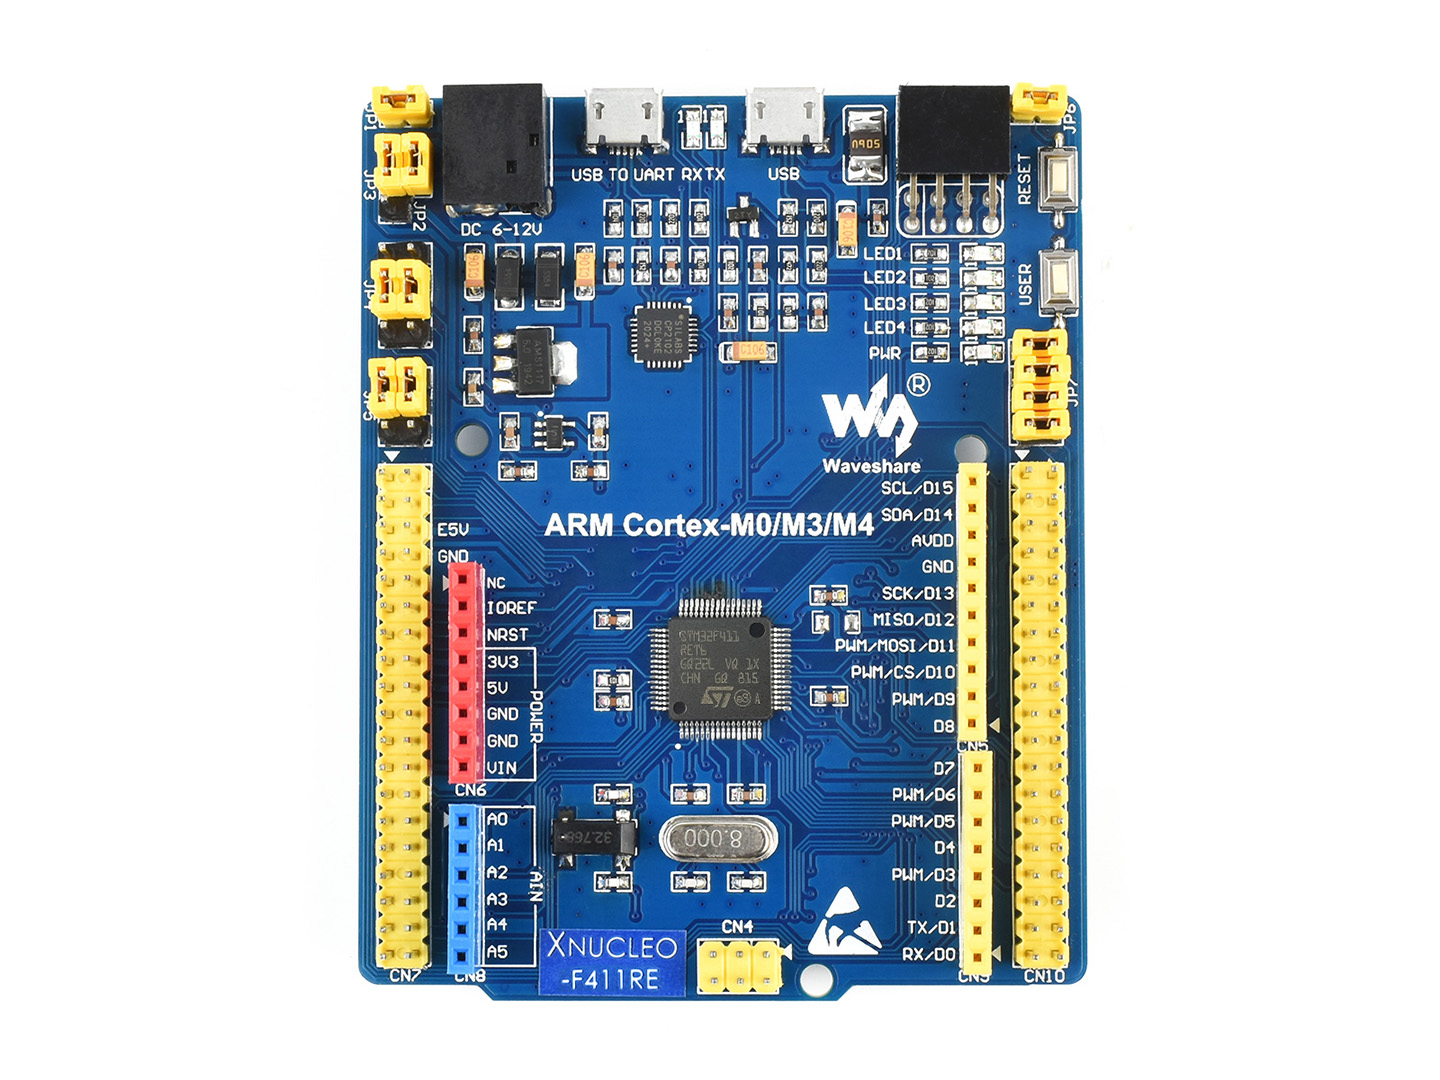
\includegraphics[width=.8\textwidth]{Figures/3_xnucleo_f411re.jpg}
	\caption{XNUCLEO-F411RE development board by Waveshare}
	\label{fig:3_xnucleo_f411re_pcb}
\end{figure}
The choice of platform for controls and data acquisition is an embedded system. A microcontroller is a small computer that is built into a single \gls{ic} chip. It includes a \gls{cpu}, memory, and \gls{io} peripherals, and it is designed to perform a specific set of tasks. Microcontrollers are used in a wide range of electronic devices, including appliances, automobiles, industrial control systems, and consumer electronics. Microcontrollers are often used in applications where a small, low-power device is needed to perform simple tasks, such as controlling a motor or reading a sensor. They are usually programmed in a high-level language, such as C or C++, and they can be programmed to perform a variety of tasks, depending on the specific application. The chosen \gls{mcu} for this project is XNUCLEO-F411RE, visible in \cref{fig:3_xnucleo_f411re_pcb}, because it is sufficient for the application and sourcing limitations within the \gls{ic} supply chain. For implementing the control system, a \gls{rtos} can offer multiple benefits for the embedded system development. A RTOS is an operating system that is designed to handle real-time applications. Real-time applications are those that require timely processing of data in order to function correctly. This can include tasks such as controlling industrial machinery, monitoring and controlling processes. Real-time operating systems are designed to prioritize certain tasks and ensure that they are completed within a specific timeframe. They do this by allocating a certain amount of processing resources to each task, and by interrupting the execution of lower-priority tasks as needed to ensure that high-priority tasks are completed on time. RTOSs typically include features such as preemptive scheduling, real-time communication, and support for multiple processors and hardware architectures. Alternatively, a vendor-locked baremetal implementation is an option, in this case, STM32 HAL. Notable differences between the two approaches are, but not limited to:
\begin{itemize}
	\item Multitasking: RTOS allows for parallel execution that enable more complex applications.
	\item Portability: Standard modules mean that the same code can be easily ported to other devices and even other platforms without modifications.
	\item Reduced development time: Especially for rapid prototype development, using pre-existing APIs significantly reduces development time by providing many of the low-level tasks such as scheduling, resource management, and timing by the operating system.
\end{itemize}

%\subsection{Development Environment}
%\begin{figure}[htbp]
%	\centering
%	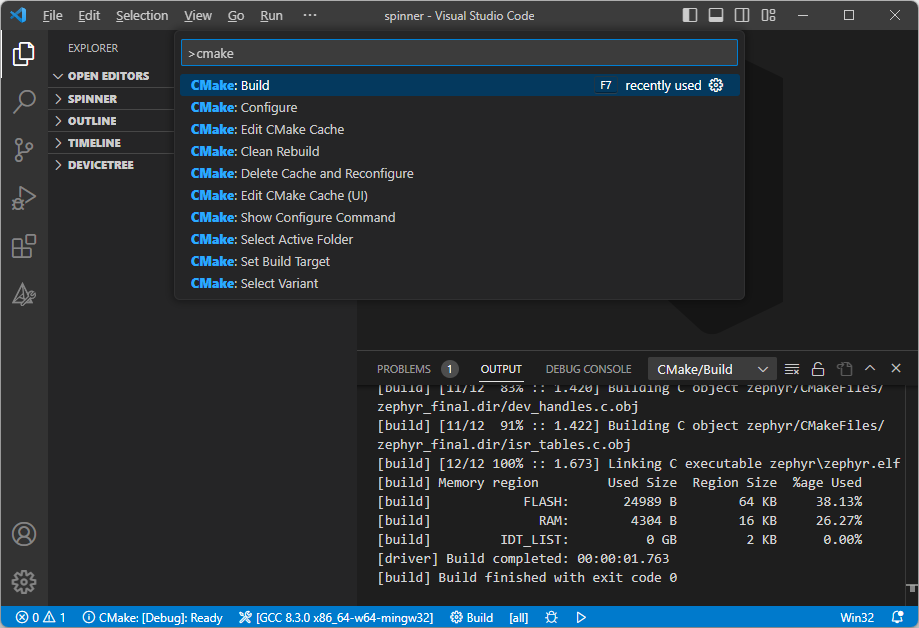
\includegraphics[width=.8\textwidth]{Figures/3_cmake_vscode.png}
%	\caption[VSCode editor with CMake Tools active]{VSCode editor with CMake Tools active, displaying available tasks}
%	\label{fig:3_vscode_cmake_build}
%\end{figure}
%
%Visual Studio Code (VSCode) is an \gls{open-source} code editor developed by Microsoft. It is designed to be highly customizable and efficient, with a wide range of features and extensions that allow developers to customize their workflows and improve their productivity. VSCode works in synergy with CMake through an extension. CMake is a cross-platform build system that helps developers manage the build process for their projects. It is used to generate build files for different platforms and build systems, to build projects on a wide range of platforms. When using CMake with VSCode, the basic idea is to use the CMake extension for VSCode to generate the appropriate build files for the target platform, and then use the VSCode tasks and debugging capabilities to build and debug the project. After setup of VSCode, the CMake Tools \cite{cmake} extension can be found in the VSCode Marketplace. The CMake Tools extension allows you to create, configure and build CMake projects from within VSCode. Once the extension is installed, you can create a new CMake project and configure it by specifying the path to the \texttt{CMakeLists.txt} file and other settings like the target platform and build configuration. After configuring the project, the VSCode tasks are provided to build and run the project. These tasks are defined in the \texttt{tasks.json} file, which can be customized to specify the build command and other options. Examples of tasks are build the project, cleaning the build directory, or running tests. The available CMake tasks are shown in \cref{fig:3_vscode_cmake_build}. In addition to building and running the project, VSCode allows for debugging capabilities to debug code.

\section{Pulse Generator}
Initially, a pulse generator was designed by using a programmable synthesizer circuit, but due to constraints within generating complementary PWM with dead-time when driving the half-bridge, a timer based PWM generation in the microcontroller is preferable. In a half-bridge power stage, dead-time refers to the amount of time that elapses between the moment when one of the switches in the half-bridge (either the high-side or the low-side switch) turns off and the moment when the other switch turns on. During the dead-time, both switches in the half-bridge are off, which means that there is no current flowing through either switch in the half-bridge. A scenario where both switches are on, can cause problems if the output of the half-bridge is connected to a load, as it may cause the load to behave erratically or even be damaged. To avoid these problems, it is important to carefully consider the amount of dead-time in a half-bridge power stage. In general, a longer dead-time will reduce the risk of damage to the load, but it will also reduce the efficiency of the power stage, as energy will be lost during the dead-time. Therefore, it is important to carefully balance the trade-off between efficiency and safety in order to determine the optimal amount of dead-time for a given half-bridge power stage. Based on discussions during design review, it was decided to change approach and generate the two complementary PWM signals by configuring the PWM module of the controller with the functionality though with a trade-off in resolution. However, for this application there is no need to amplitude modulate the output signal.
In the context of a PW Doppler system, it is desired to generate 4 signals:
\begin{itemize}
	\item \qty{5}{\mega\hertz} complementary signal \texttt{PWM} with dead-time for the pulsed burst during transmit mode.
	\item \qty{5}{\mega\hertz} complementary signal \texttt{PWMN} with dead-time and opposite phase from \texttt{PWM}.
	\item \qty{10}{\kilo\hertz} signal \texttt{PRF} for the timing control of the transmit/receive switch.
	\item \qty{20}{\mega\hertz} clock signal \texttt{CLK} for the demodulation circuit in the receiver.
	\item \texttt{PULSE} and \texttt{GATE} controlled by \texttt{PRF} for S/H control with pulse length $t_{\mathrm{pulse}} = N_{\mathrm{pulse}} \times T_{\mathrm{prd}}$, where $T_{\mathrm{prd}} = \sfrac{1}{f_{\mathrm{pwm}}}$. \texttt{GATE} is delayed from pulse by \texttt{sample depth}.
\end{itemize}

\begin{figure}[htbp]
	\centering
	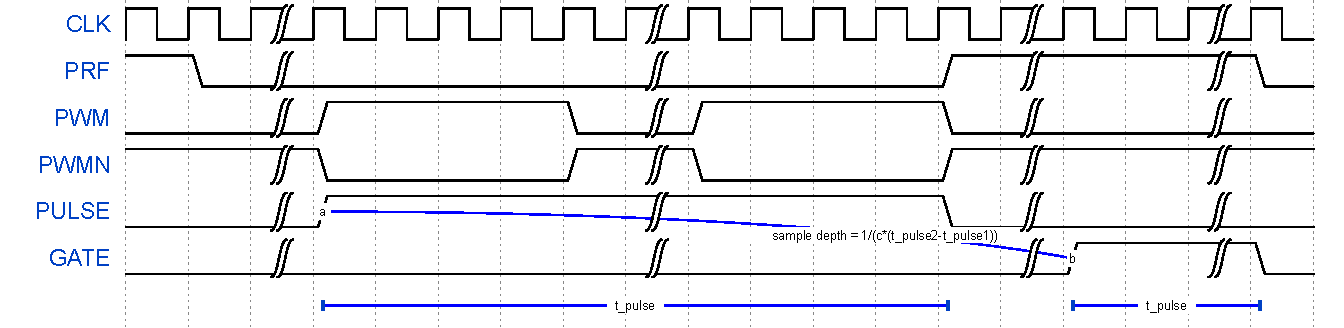
\includegraphics[width=\textwidth]{Figures/3_wavedrom.pdf}
	\caption{Timing diagram of various control signals for an arbitrary $n$ length pulse chain expressed by the second diagram gap}
	\label{fig:3_pulse_timing_diagram}
\end{figure}

\begin{figure}[htbp]
	\centering
	\resizebox{\textwidth}{!}{%
    \begin{tikzpicture}[
	node distance = 20mm and 20mm,
	V/.style = {draw, fill=gray!10},
	G/.style = {draw, fill=white},
	every edge quotes/.style = {auto, font=\footnotesize, sloped}
	]
	\begin{scope}[nodes=V]
		\node (1)   {Transducer};
		\node (2) [below=10mm of 1]    {TR Switch};
		%\node (3) [right=of 2]          {3};
		\node (4) [right=of 2]    {Pulse Generator};
		%\node (5) [below left=of 4]    {5};
		\node (6) [below=of 2]          {Power Stage};
		%\node (7) [right=of 4]          {Control System};
		%\node (8) [right=of 7]          {Inputs};
		\node (9) [above=10mm of 4]      {Demodulator};
		\node (10) [right=of 4]     {Time Delay};
		\node (11) [above=10mm of 10]     {Sample and Hold};
	\end{scope}
	\draw   (1)  edge[""] (2)
	%       (2)  edge["B"] (3)
	%      (3)  edge["C"] (4)
	(4)  edge["PWM/PWMN"] (6)
	(2)  edge["PRF"] (4)
	(6)  edge["HV PULSES"] (2)
	(4)  edge["CLK"]   (9)
	(4)  edge["PULSE"] (10)
	(10) edge["GATE"] (11);
	%
	%       (4)  edge["G"] (7)
	%       (7)  edge["H"] (8);
\end{tikzpicture}
}%
\end{figure}

\section{Power Stage}
%\begin{figure}[htbp]
%	\centering
%	\resizebox{.6\textwidth}{!}{%
%		\begin{circuitikz}
%			\tikzstyle{every node}=[font=\LARGE]
%			\draw (7,12) to[Tnmos] (7,14);
%			\draw (6.15,13) to[short] (6,13);
%			\draw (7,16) to[Tpmos] (7,18);
%			\draw (6.15,17) to[short] (6,17);
%			\draw (5.5,16.5) to[R,l={ \normalsize $R1$}] (5.5,17.75);
%			\draw (5,16.5) to[empty Zener diode,l={ \normalsize $D1$}] (5,17.75);
%			\draw (5,13) to[empty Zener diode,l={ \normalsize $D2$}] (5,11.75);
%			\draw (5.5,13) to[R,l={ \normalsize $R2$}] (5.5,11.75);
%			\draw [](5,17.75) to[short] (7,17.75);
%			\draw [](7,17.75) to[short] (7,17.5);
%			\draw[] (6,16.5) to[short] (5,16.5);
%			\draw[] (6,13) to[short] (5,13);
%			\draw [](7,12) to[short] (7,11.75);
%			\draw[] (7,11.75) to[short] (5,11.75);
%			\draw (5.5,13) to[short, -*] (5.5,13);
%			\draw (5.5,11.75) to[short, -*] (5.5,11.75);
%			\draw (5.5,17.75) to[short, -*] (5.5,17.75);
%			\draw (5.5,16.5) to[short, -*] (5.5,16.5);
%			\draw [ -Stealth] (7,17.75) -- (7,18.25);
%			\draw [ -Stealth] (7,11.75) -- (7,11.25);
%			\draw [](5,16.5) to[short, -o] (4.25,16.5);
%			\draw [](5,13) to[short, -o] (4.25,13);
%			\draw (7,15.5) to[D,l={ \normalsize $D3$}] (8.25,15.5);
%			\draw (8.25,14) to[D,l={ \normalsize $D4$}] (7,14);
%			\draw [](8.25,14.75) to[short, -o] (9.25,14.75);
%			\draw [](8.25,14) to[short] (8.25,15.5);
%			\draw (8.25,14.75) to[short, -*] (8.25,14.75);
%		\end{circuitikz}
%	}%
%
%	\label{fig:my_label}
%\end{figure}
\begin{figure}[htbp]
	\centering
	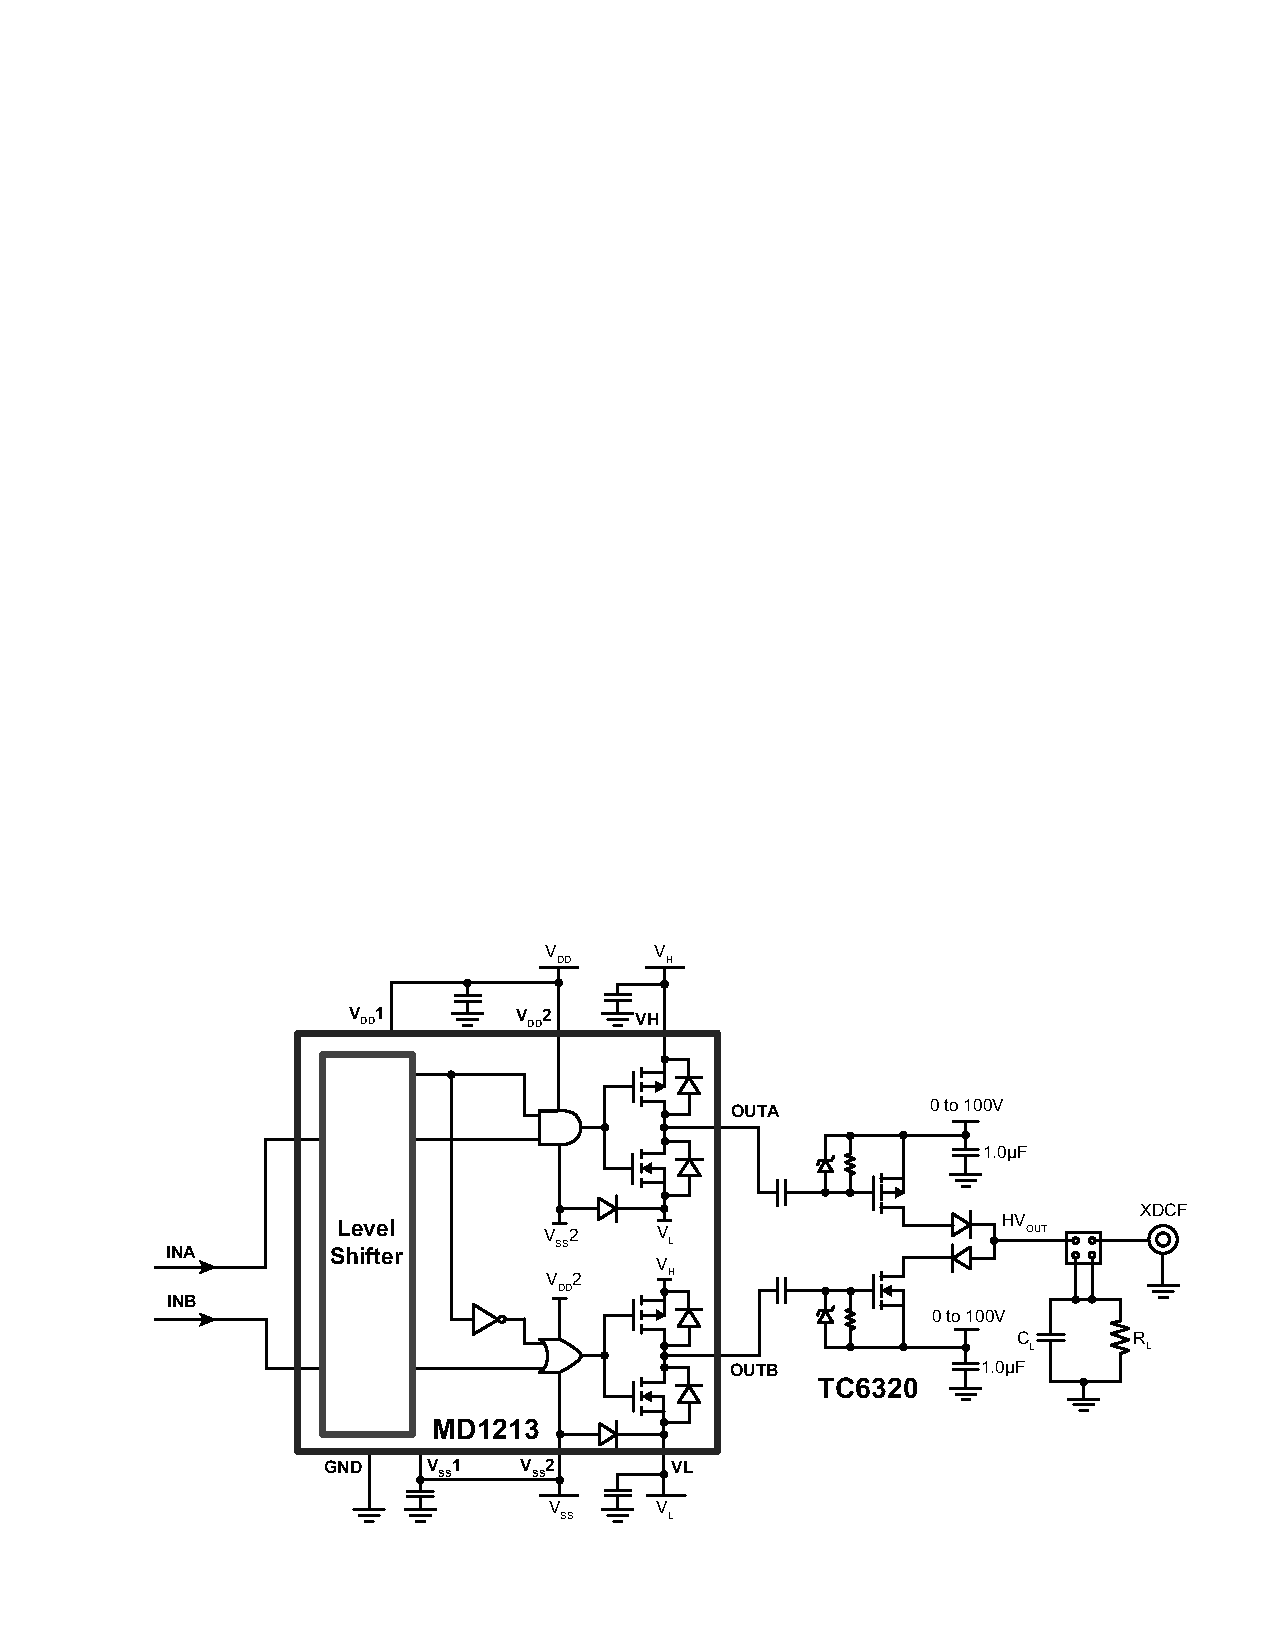
\includegraphics[width=\textwidth]{Figures/3_power_stage_block.pdf}
	\label{fig:3_power_stage}
	\caption[Block diagram of power stage]{Block diagram of power stage \cite{MD1213DB1}}
\end{figure}
Several MOSFET drivers were considered, e.g. ISL55111\cite{ISL55111}, EL7104\cite{EL7104}, and MD1213\cite{MD1213}. The MD1213 has an advantage over the ISL55111 or EL7104 for ultrasound MOSFET drivers since it is specifically designed for high-voltage P-channel and N-channel MOSFETs in medical ultrasound and other applications needing a high output current for a capacitive load. It has a high-speed input stage with a logic interface that can function from \qtyrange{1.8}{5}{\volt} and an ideal operating input signal range of \qtyrange{1.8}{3.3}{\volt}. The DC-coupled adaptive threshold circuit sets the level translator switch threshold to the average of the input logic \gls{low} and logic \gls{high} levels. Consequentially, the MD1213 is designed primarily for driving MOSFETs in medical ultrasound applications, whereas the ISL55111 and EL7104 are more general-purpose drivers that may not perform as well in ultrasound applications. The MD1213's output stage has a distinguishing feature in that the \gls{low} and \gls{high} levels of the output signal may be set independently of the rest of the circuit's supply voltages. The input logic levels, for example, might be \qty{0}{\volt} and \qty{1.8}{\volt}, whereas the control logic is powered by \qtyrange[retain-explicit-plus]{+5}{-5}{\volt}. The output \gls{low} and \gls{high} values, on the other hand, may be changed between \qtyrange[retain-explicit-plus]{-5}{+5}{\volt}. This gives you greater flexibility in adjusting the output signal levels to meet individual needs. The output stage may also provide peak currents of up to \qty{2}{\ampere}, depending on the load capacitance and supply voltages employed. Seen in \cref{fig:3_power_stage} is the circuit diagram of the power stage with the gate driver on the left side and the half-bridge on the right side.
\begin{figure}[htbp]
	\centering
	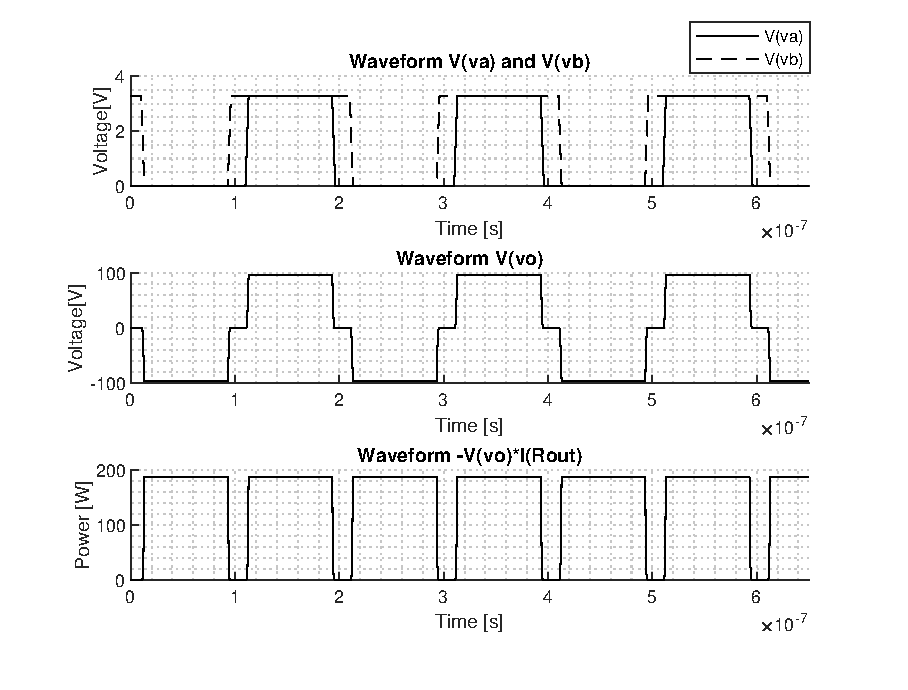
\includegraphics[width=.8\textwidth]{Figures/3_transmitter_sim_out.eps}
	\caption[LTspice simulation output of transmitter]{LTspice simulation output of transmitter with level shifter and half-bridge power stage from \cref{fig:app_ltspice_transmitter}}
	\label{fig:3_transmitter_sim}
\end{figure}
Using a \gls{spice} macro model, an LTspice simulation of the power stage was implemented where the full model can be seen in \cref{fig:app_ltspice_transmitter}. The resulting waveforms are seen in \cref{fig:3_transmitter_sim}. In the top subplot, the input voltages \texttt{INA} and \texttt{INB} are seen with their dead-time visible on each overlapped on period. Since \texttt{INB} is driving an N-channel \gls{mosfet}, the driving pulse train should be thought of as having the opposite polarity. When looking at the middle subplot, it is noted that dead time is visible as the time when the output voltage is zero. Thus, during that time neither \gls{fet} are allowing a current to pass, and therefore the voltage across the load is equal to zero. The lower subplot shows the maximum ideal power delivery using the peak pulse voltage, assuming the load is equal to \qty{50}{\ohm}. In reality, due to the laboratory instruments available for experiments, the pulse peak voltage will be less than $\pm \qty{100}{\volt}$.

\section{Transmit/Receive Switch}
\begin{figure}[htbp]
	\centering
%	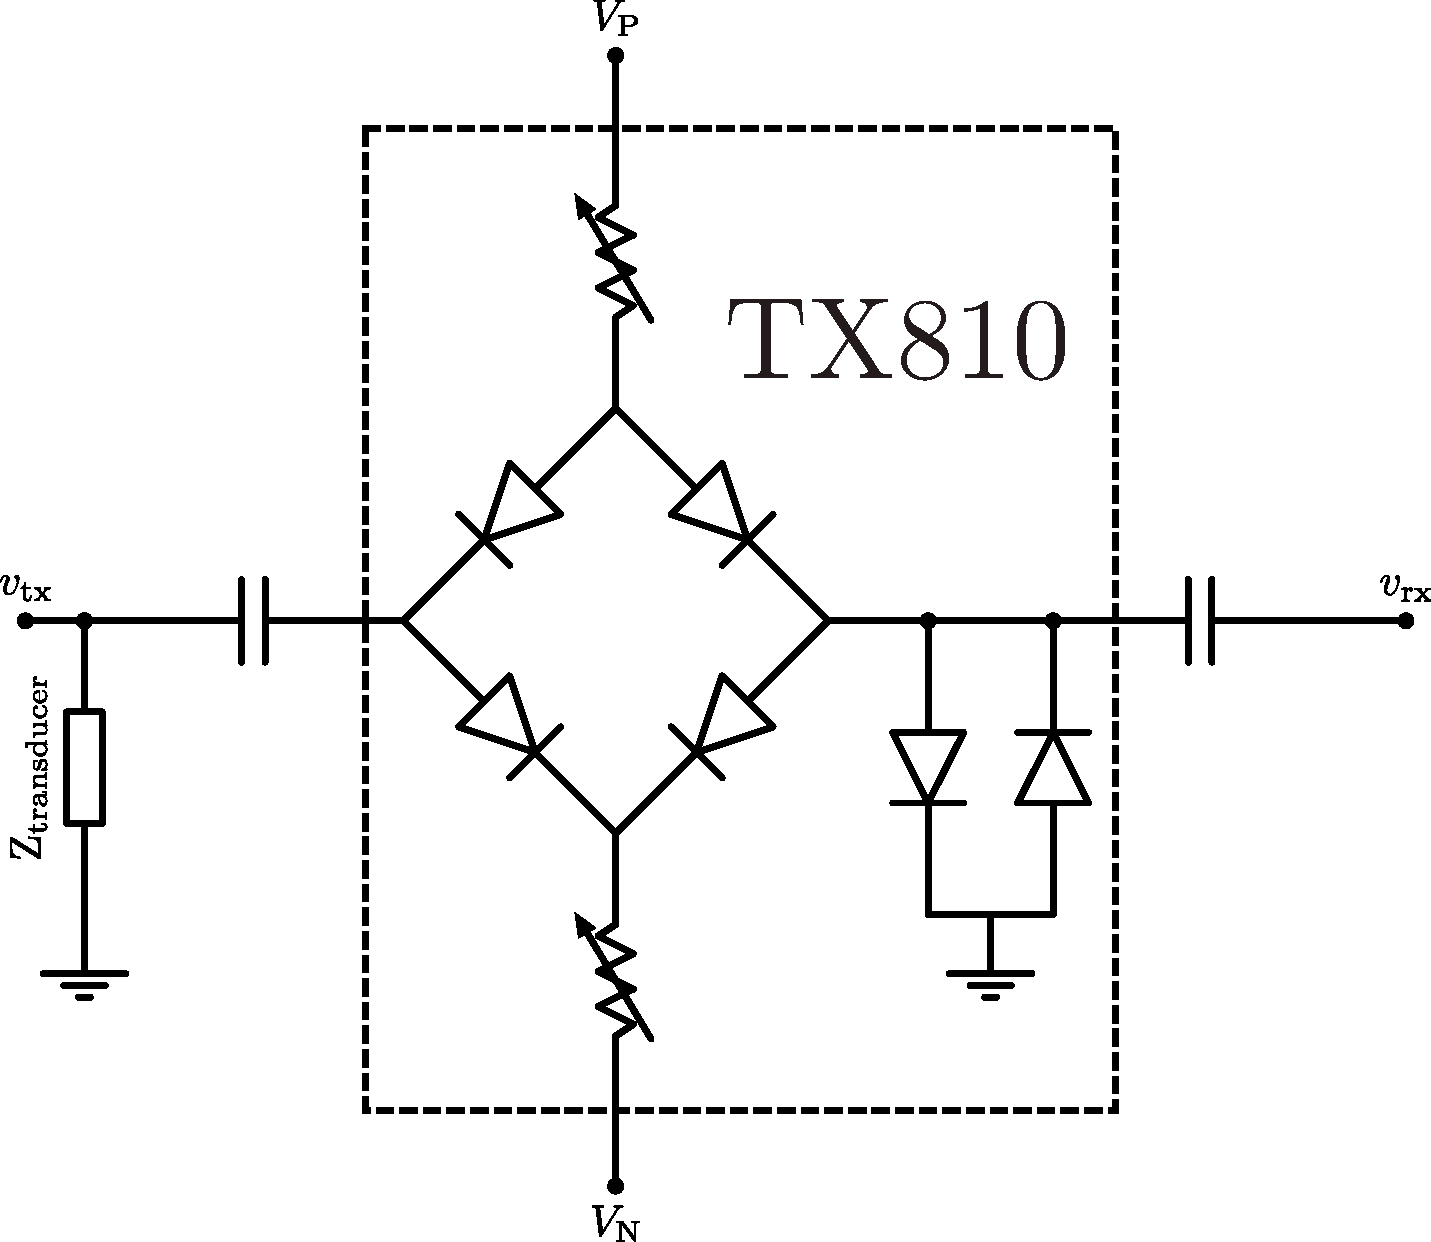
\includegraphics[width=.8\textwidth]{circuits/switch.pdf}
	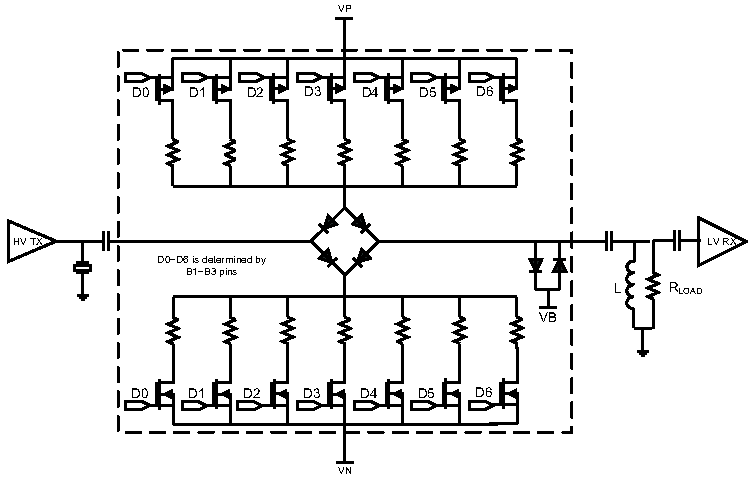
\includegraphics[width=.8\textwidth]{Figures/3_switch_tx810_block.pdf}
	\caption[Block diagram of TX/RX switching circuit]{Block diagram of TX/RX switching circuit where the inputs D1 through D6 are binary decoded from inputs $B_1$, $B_2$, $B_3$ \cite{TX810}}
	\label{fig:3_switch}
\end{figure}
Among the design considerations for the transmit and receive switch were the TX810\cite{TX810} and MD0101\cite{MD0101}. Both ICs are acceptable choices, however, the MD0101 is a newer and generally better choice since it has a lower insertion loss, which means that less of the ultrasound signal is lost as it passes through the switch. This results in a higher-quality image with a better signal-to-noise ratio. Additionally, MD0101 has a wider bandwidth, which means that it can transmit and receive ultrasound signals over a broader range of frequencies. However, since the TX810 is in stock and is also acceptable, it was chosen for the design. TX810 is an IC from Texas Instruments that can be used to switch transmit and receive paths of an ultrasound system. The IC fundamentally works by having a 3-bit programmable pin interface that will open and close the switch with a variable bias current. See \cref{fig:3_tx810_timing} for a visualisation of the switching operation, where \texttt{INPUT} is the incoming Doppler waveform being picked up from the transducer, \texttt{B3/B2/B1} is the switching signal closing the switch and thereby going in receive mode, and \texttt{OUTPUT} is the received signal seen in the \gls{afe}. When high-voltage transmitter signals are applied to the input, the internal diodes limit the output voltage. While in receive mode, the TX810's insertion loss is minimized. The TX810 features a 3-bit interface that may be used to program bias current from \qty{7}{\milli\ampere} to \qty{0}{\milli\ampere} for varying performance and power requirements, unlike conventional T/R switches. The device is put up in power-down mode when the TX810 bias current is set to \qty{0}{\milli\ampere} (high-impedance mode). The TX810 does not put a significant load on high-voltage transmitters when operating in the high-impedance mode.
\begin{figure}[htbp]
	\centering
	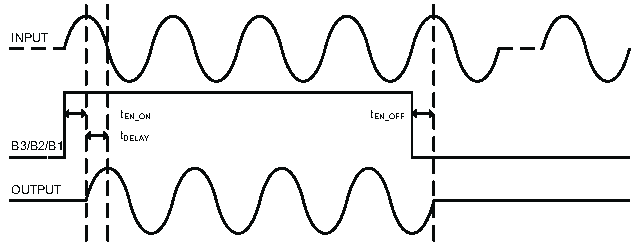
\includegraphics[width=.8\textwidth]{Figures/3_tx810_timing.pdf}
	\caption[Timing diagram of switching interface]{Timing diagram of switching interface where $t_{\mathrm{EN\_ON}}=\qty{0.6}{\micro\second}$, $t_{\mathrm{EN\_OFF}}=\qty{2.4}{\micro\second}$, and $t_{\mathrm{DELAY}}=\qty{1.3}{\nano\second}$ for the condition $B_1=B_2=B_3$ \cite{TX810}}
	\label{fig:3_tx810_timing}
\end{figure}

\begin{figure}[htbp]
	\centering
	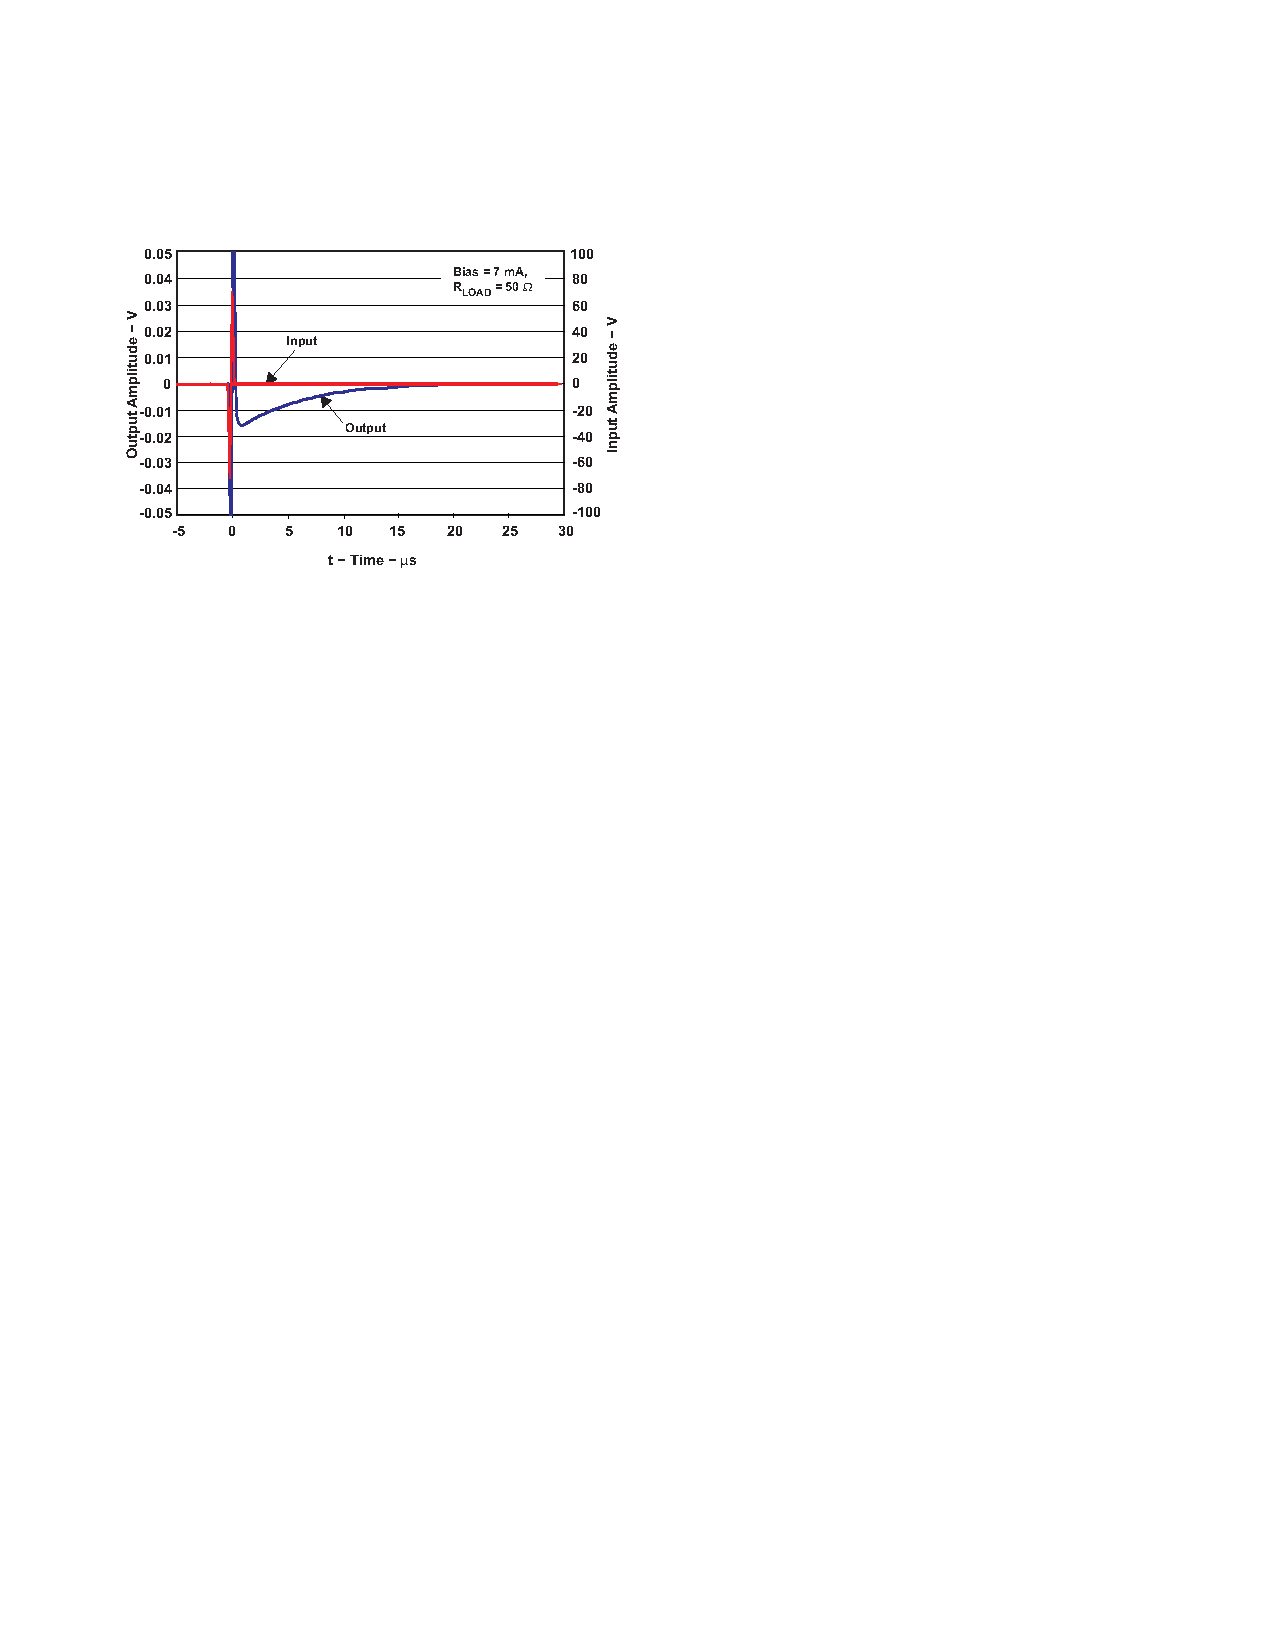
\includegraphics[width=.8\textwidth]{Figures/3_tx810_recovery.pdf}
	\caption[Recovery time from transmitting to receiving state with an AC coupled high-voltage pulse and TX810]{Recovery time from transmitting to receiving state with an AC coupled high-voltage pulse and TX810 \cite{TX810}}
	\label{fig:3_switch_recovery}
\end{figure}
Seen in \cref{fig:3_switch_recovery} is the recovery time between transient states in the TX810 diode bridge where the red curve is the input and blue is the output signal. According to the specified output curve, it takes approximately \qty{15}{\micro\second} to recover from the transmitting pulse. Thus, back-calculating to find the minimum distance to reliably receive an undisturbed signal is proportional to \cref{eq:tx810_recovery}.
\begin{subequations} \label{eq:tx810_recovery}
\begin{align}
	d &= \frac{c \cdot t}{2} \Longrightarrow \\
	d &= \frac{\qty{1480}{\meter\per\second} \cdot \qty{15}{\micro\second}}{2} = \qty{11.55}{\milli\meter}
\end{align}
\end{subequations}
Where $d$ is equal to the travel distance from the transducer to the scatterer, $c$ is the speed of sound in water (assumed to be \qty{1480}{\meter\per\second}), and $t$ is the recovery time as specified in  \cref{fig:3_switch_recovery}. The reason for dividing the distance by half is because the travel time is double the distance since the acoustic wave has to travel the distance from the transducer and the reflected wave has to travel back the equal distance. This means that a distance of less than \qty{11.55}{\milli\meter} to a scatterer is likely to produce an unreliable measurement. The ultrasound switch is designed to switch the transmit and receive paths at specific times, as determined by the input signals. A PCB design was implemented in Altium Designer \cite{altium} utilising three channels of the maximum eight available channels in the IC. Seen in \cref{fig:3_ultrasoundswitch} is a 3D render of the designed PCB.

\begin{figure}[htbp]
	\centering
	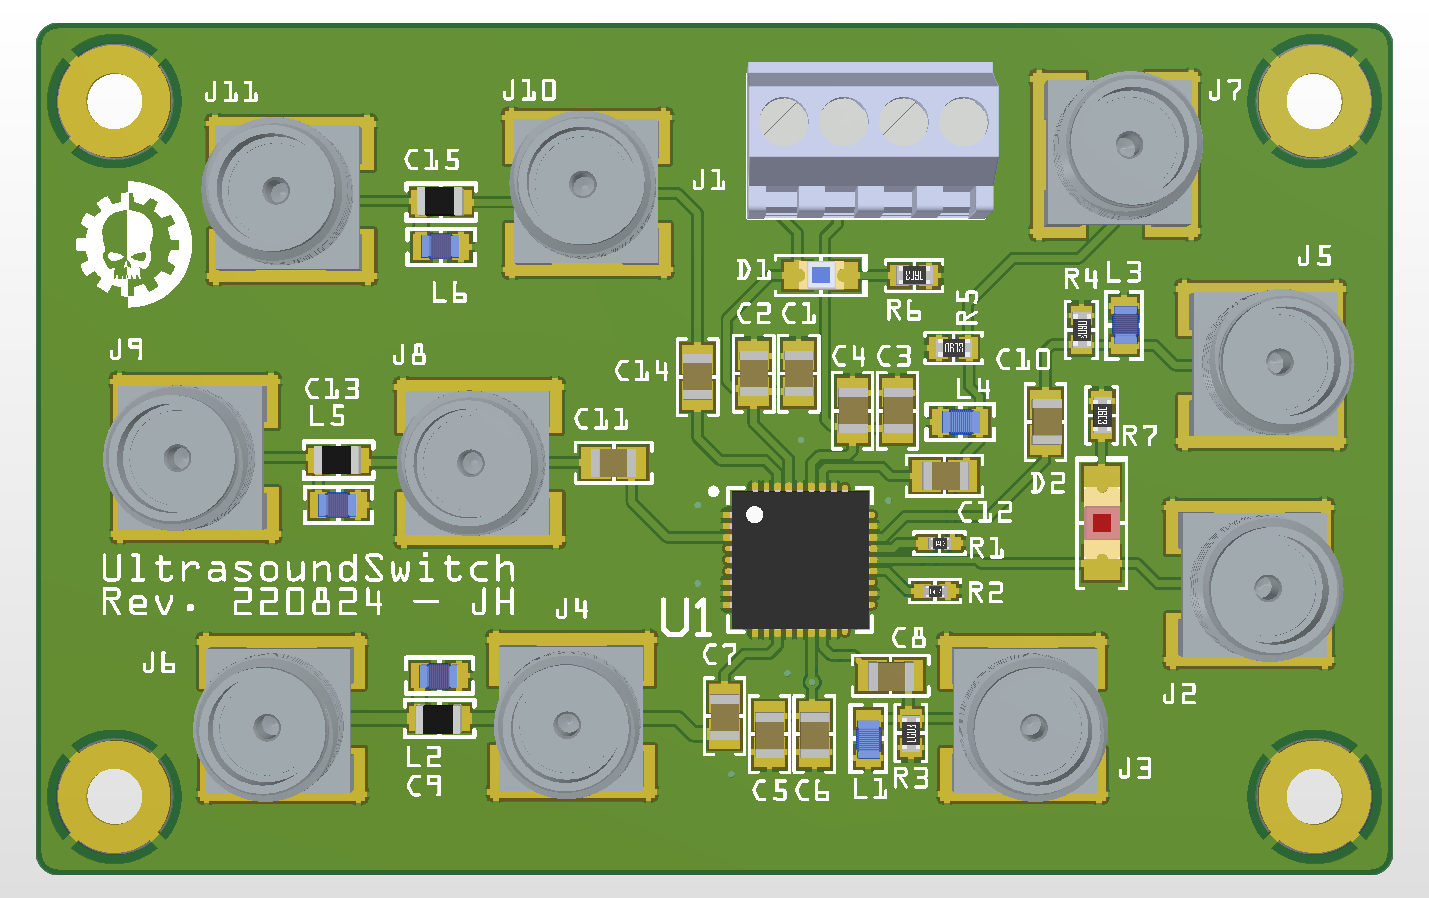
\includegraphics[width=.8\textwidth]{Figures/3_ultrasoundswitch.png}
	\caption{3D Render of PCB in Altium Designer}
	\label{fig:3_ultrasoundswitch}
\end{figure}
The module is designed with three usable channels, either three separate transducers for multi-angle sonography, or a \gls{cmut} with three channels in a single angle. However, in the following experiments with the TX/RX switch, only one channel will be used for simplifying the data acquisition experiments.

\section{Band-pass Filter}
\begin{figure}[htbp]
	\centering
	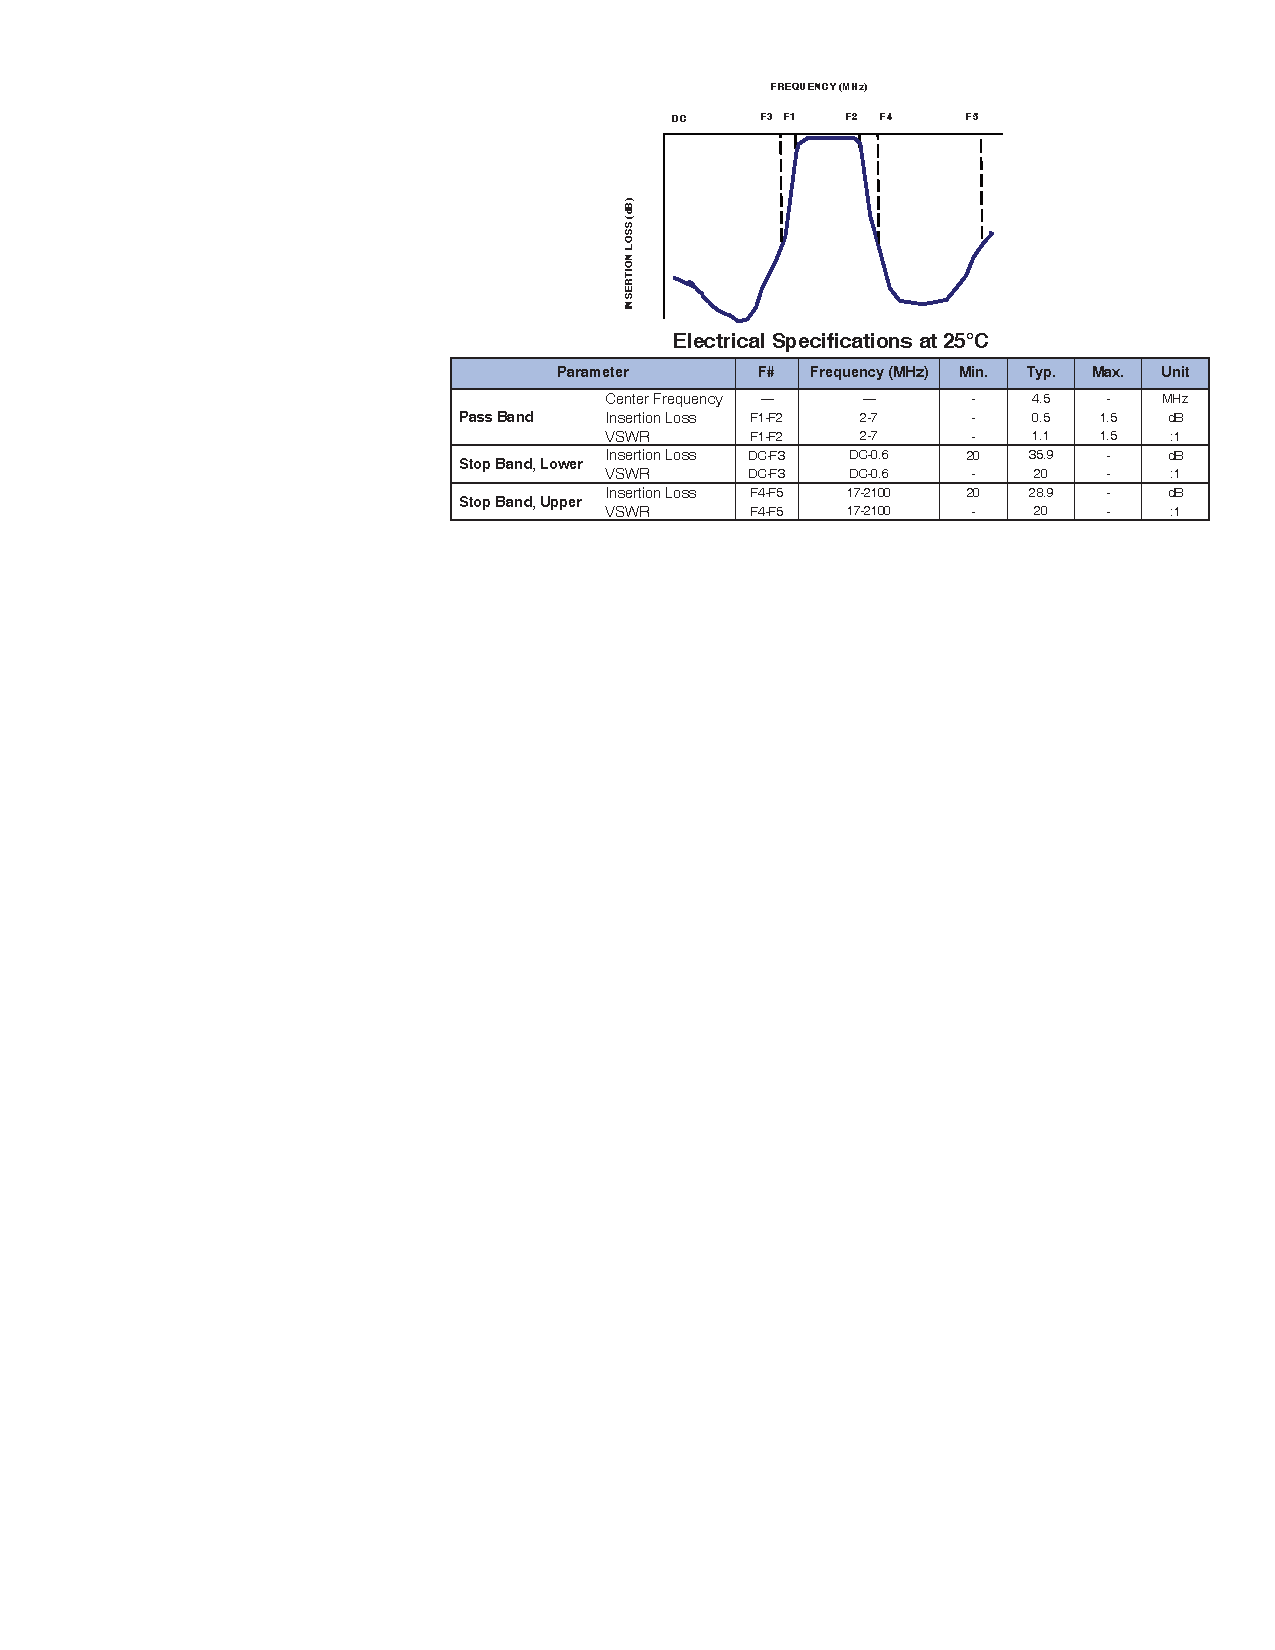
\includegraphics[width=\textwidth]{Figures/3_bpf_specs.pdf}
	\caption[Band-Pass Filter insertion loss and specifications]{Band-Pass Filter with (above) insertion loss showing a pass band of \qtyrange{2}{7}{\mega\hertz} of \qty{0.5}{\decibel} insertion loss and (below) electrical specifications showing the minimum stopband attenuation of \qty{20}{\decibel} \cite{BPF}}
	\label{fig:3_bpf_specs}
\end{figure}
After the signal is received, it is filtered with a \gls{bp} filter to remove unwanted noise and interference from the received signal. The presence of these unwanted frequency components can distort the received signal and reduce the quality of the resulting imaging. The specs from the datasheet of used modular component BPF-C4R5+ \cite{BPF} are seen in \cref{fig:3_bpf_specs}. Filtering the received signal through this device means that any signals produced by the transducer at frequencies outside the range of interest will be attenuated. An ultrasound receiver requires a band-pass filter to enable only the frequencies within a predetermined range to pass through while blocking out frequencies outside that range. Using the specs and S21 forward transmission coefficient data, a bode plot can be visualised in \cref{fig:3_bpf_s21_bode_plot}.

\begin{figure}[htbp]
	\centering
	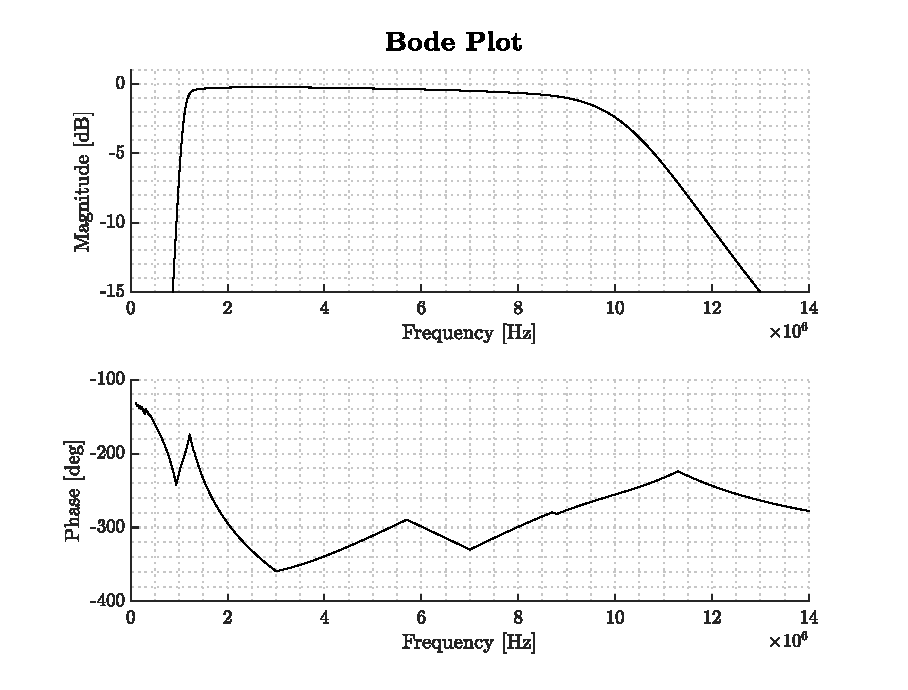
\includegraphics[width=.8\textwidth]{Figures/3_bpf_s21_vals.eps}
	\caption[Bode plot of bandpass filter]{Bode plot of BPF-C4R5+ S21 forward transmission coefficient of the active filter as specified by the manufacturer}
	\label{fig:3_bpf_s21_bode_plot}
\end{figure}

\section{Preamplifier}
\begin{figure}[htbp]
	\centering
	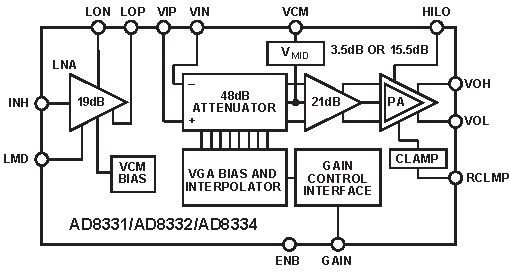
\includegraphics[width=.8\textwidth]{Figures/3_ad8332_block.pdf}
	\caption[Block diagram of preamplifier AD8332]{Block diagram of preamplifier AD8332 \cite{AD8332}}
	\label{fig:3_preamplifier_block}
\end{figure}
The isolated signal is still rather weak to be measured using digital circuits, and therefore the amplitude must be increased with the preamplifier circuit. This circuit is based on the integrated circuit from Analog Devices AD8332 \cite{AD8332}, which is a device that combines a dual-channel \gls{lna} and \gls{vga}, designed specifically for ultrasound systems. A diagram of its internal functional blocks can be seen in \cref{fig:3_preamplifier_block}. The AD8332 functions at frequencies up to \qty{120}{\mega\hertz}. Each channel includes an ultralow noise preamp (\gls{lna}), a \gls{vga} with \qty{48}{\decibel} of gain range, and a selectable gain post amp with adjustable output limiting. The LNA gain is \qty{19}{\decibel} with a single-ended input and differential outputs. To match the signal source without sacrificing noise performance, the LNA input impedance can be adjusted using a single resistor. The VGA has low output-referred noise, which is useful in driving high-speed differential ADCs. The gain of the post amp can be pin-selected to \qty{3.5}{\decibel} or \qty{15.5}{\decibel}, depending on the converter requirements. The output can be limited to a user-defined clamping level to avoid input overload to a subsequent \gls{adc}, with the clamping level adjusted using an external resistor. A SPICE macro model is provided by the vendor and the preamplification is successfully simulated using LTspice with the full LTspice model found in \cref{fig:app_ltspice_preamp}, and the probed inputs and outputs seen in \cref{fig:3_preamplifier_sim}.

\begin{figure}[htbp]
	\centering
	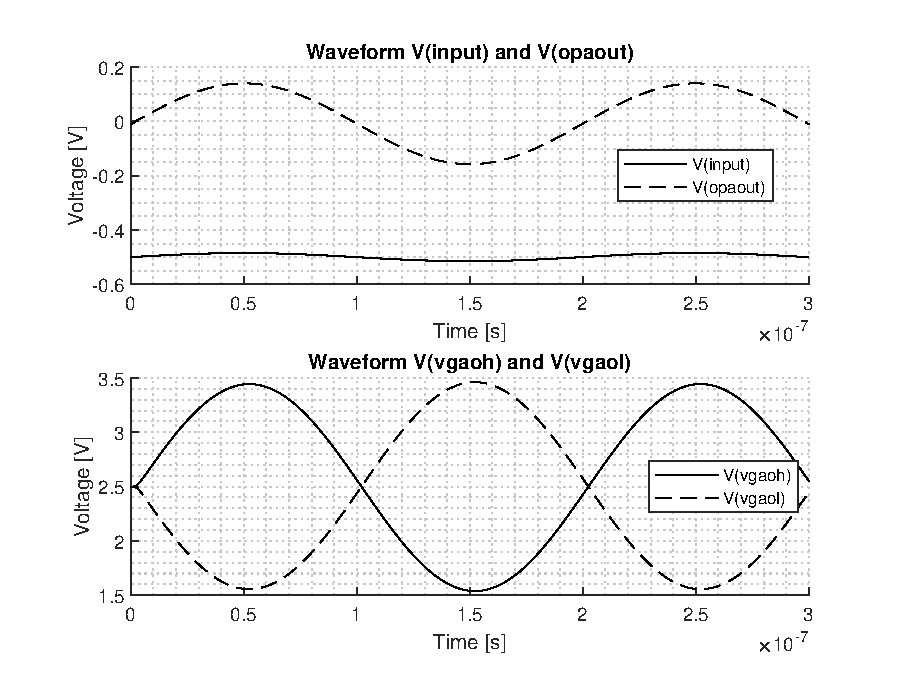
\includegraphics[width=.8\textwidth]{Figures/3_preamplifier_sim_out.eps}
	\caption[LTspice simulation output of preamplifier]{LTspice simulation output of preamplifier \gls{lna} and \gls{vga} from \cref{fig:app_ltspice_preamp}}
	\label{fig:3_preamplifier_sim}
\end{figure}

\section{Quadrature Demodulator}
\begin{figure}[htbp]
	\centering
	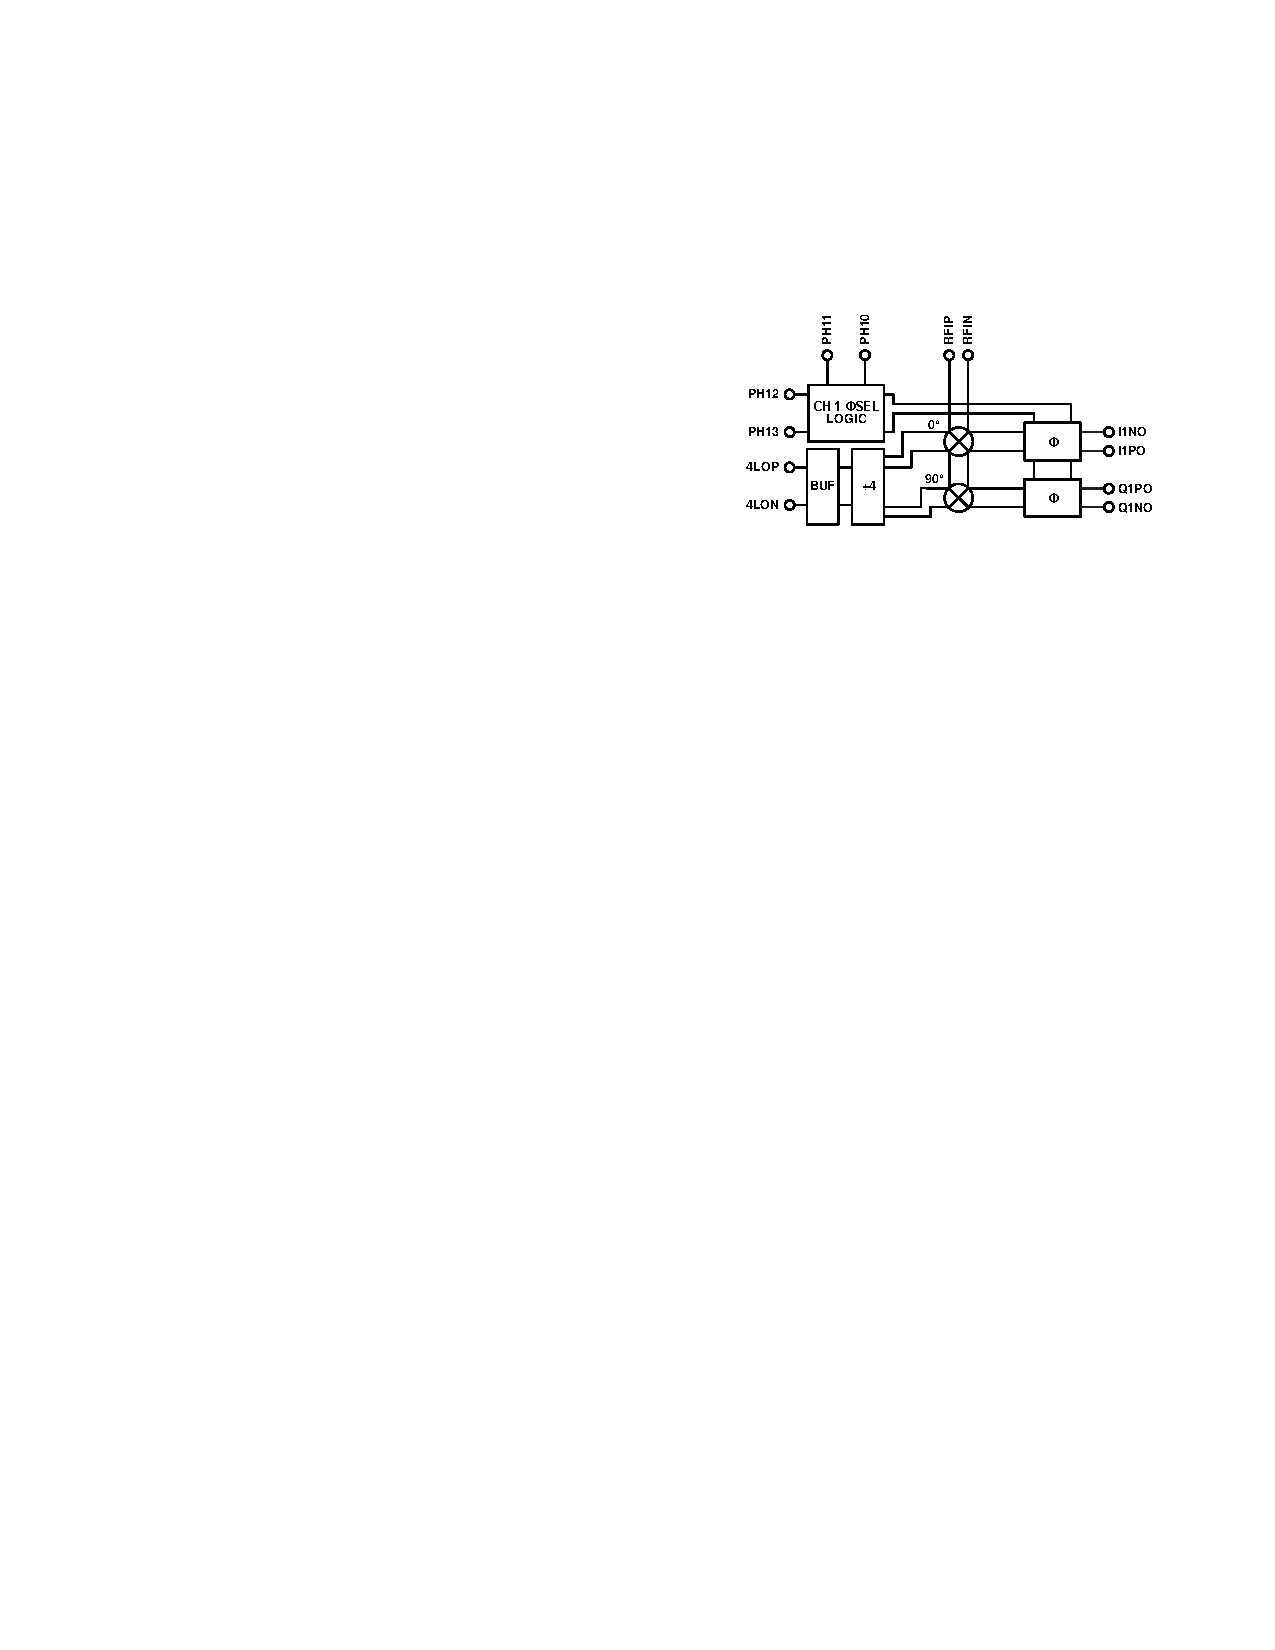
\includegraphics[width=.8\textwidth]{Figures/3_ad8333_block.pdf}
	\caption[Block diagram of demodulator AD8333]{Block diagram of demodulator AD8333 \cite{AD8333}}
	\label{fig:3_demodulator_block}
\end{figure}
After the preamplifier, the amplified signal must be demodulated to prepare it for sampling. The device used for quadrature demodulation is an integrated circuit from Analog Devices AD8333 \cite{AD8333} I/Q demodulator. A diagram of the internal functional blocks can be seen in \cref{fig:3_demodulator_block} where the primary inputs are \texttt{RFIP} and \texttt{RFIN}, which are the two differential RF signals from the preamplifier. The RF inputs connect directly to the outputs of the LNA of the preamplifier. The internal \qty{0}{\degree} and \qty{90}{\degree} phases of the local oscillator (LO) are generated by a divide-by-4 circuit that drives the mixers of a matched I/Q demodulator pair. The I and Q outputs are presented as currents, making summation possible. The summed current outputs are then converted to voltages by a high dynamic range, current-to-voltage (I-V) converter, such as the AD8021 \cite{AD8021}, which functions as a trans-impedance amplifier. A SPICE macro model is provided by the vendor and the I/Q demodulation is successfully simulated using LTspice using the LTspice model found in appendix \cref{fig:app_ltspice_demod}, with the probed inputs and outputs seen in \cref{fig:3_demod_sim_in,fig:3_demod_sim_out}.

\begin{figure}[htbp]
	\centering
	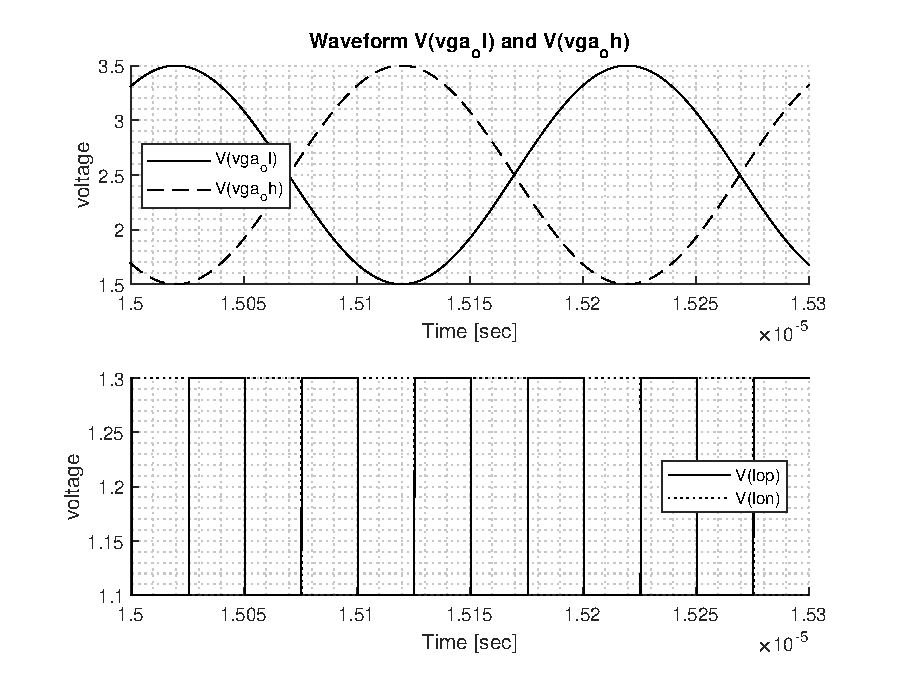
\includegraphics[width=.8\textwidth]{Figures/3_demod_sim_in.eps}
	\caption[LTspice simulation demodulator input variables]{LTspice simulation demodulator input variables from \cref{fig:app_ltspice_demod}}
	\label{fig:3_demod_sim_in}
\end{figure}
\begin{figure}[htbp]
	\centering
	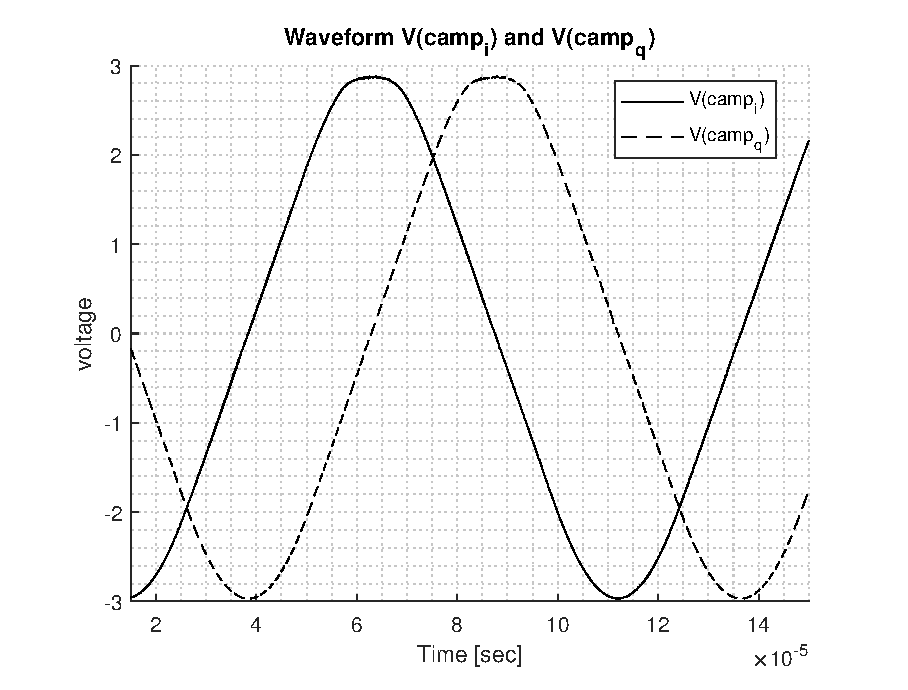
\includegraphics[width=.8\textwidth]{Figures/3_demod_sim_out.eps}
	\caption[LTspice simulation demodulator output variables]{LTspice simulation demodulator output variables Q and I voltages from \cref{fig:app_ltspice_demod}}
	\label{fig:3_demod_sim_out}
\end{figure}
\section{Sample and Hold}
\begin{figure}[htbp]
	\centering
	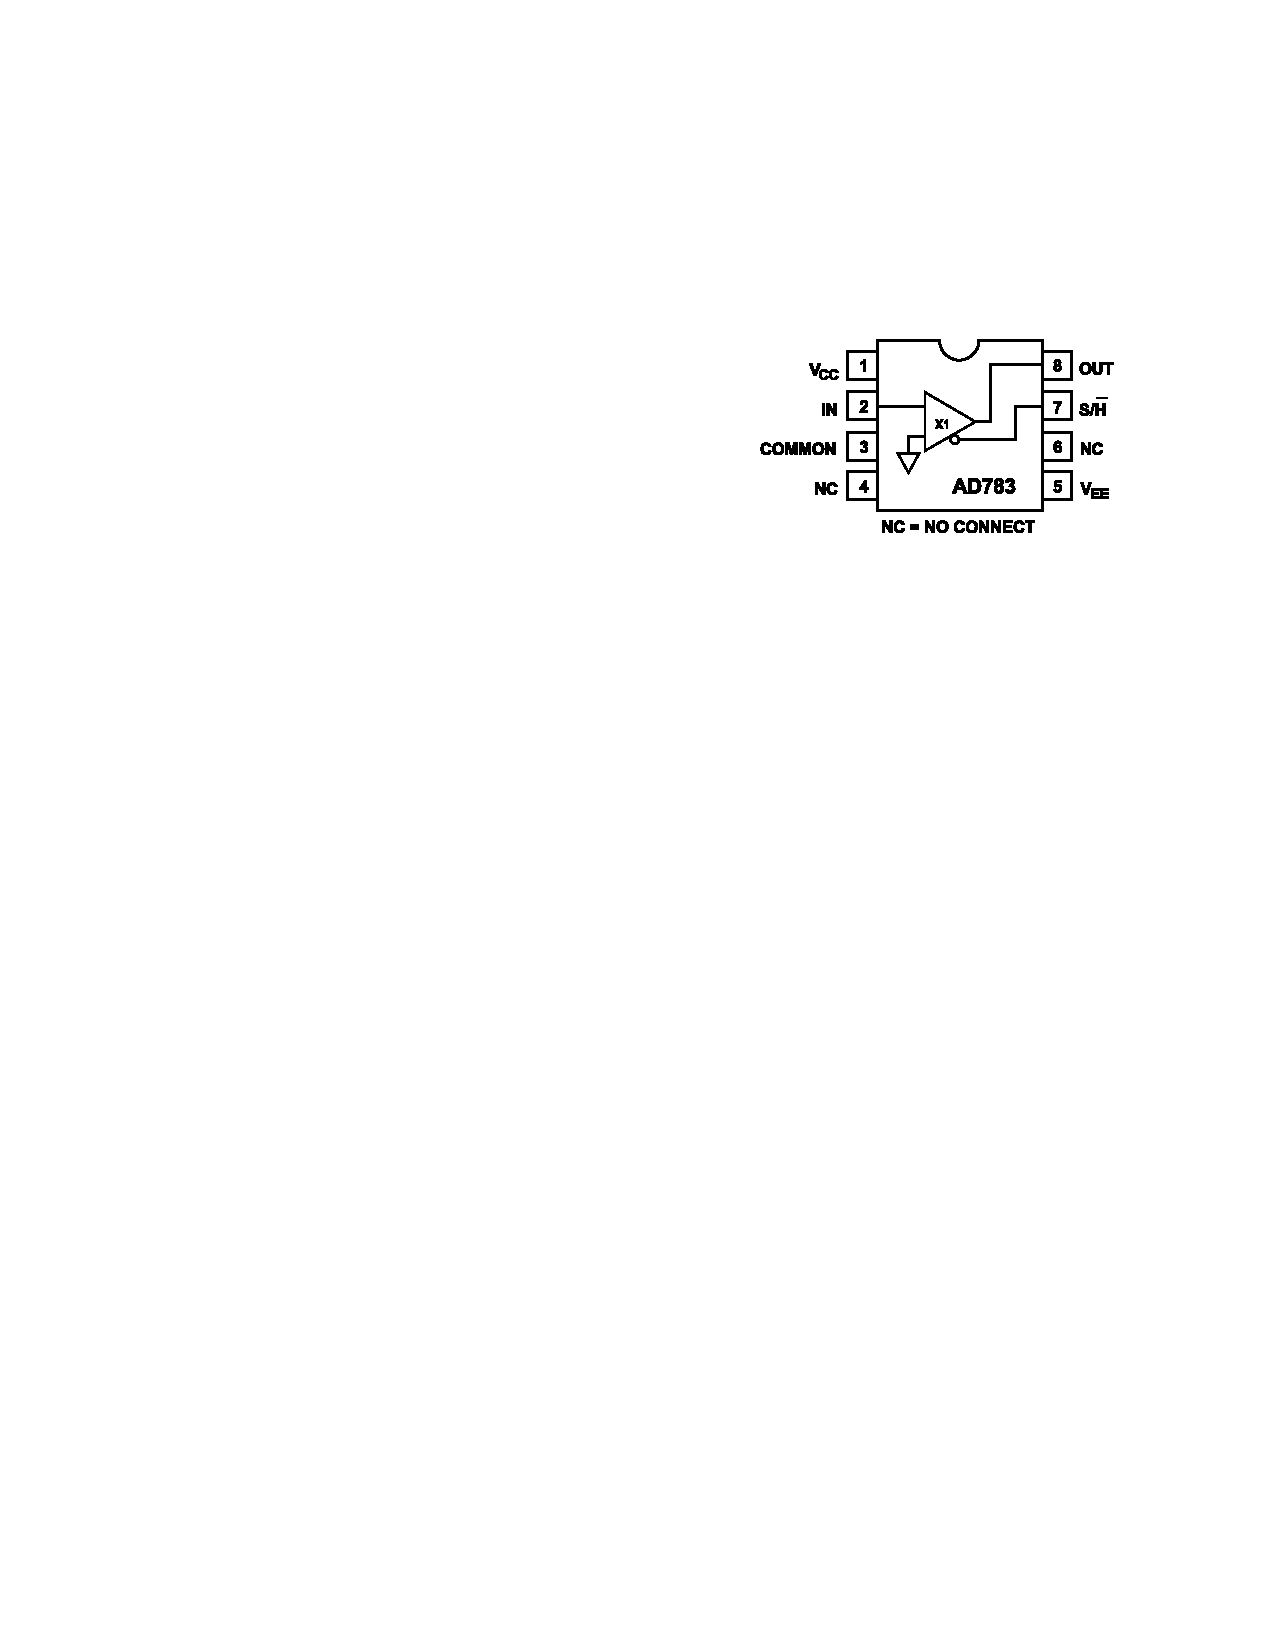
\includegraphics[width=.8\textwidth]{Figures/3_sample_hold_ad783.pdf}
	\caption[AD783 Sample and Hold amplifier block diagram]{AD783 Sample and Hold Amplifier functional block diagram \cite{AD783}}
	\label{fig:3_sha_block}
\end{figure}
In this system, the sample-and-hold amplifier is necessary to keep values between each sample line. In chapter 2, it was described how the pulsed-wave flow-meter measures the movement of scatterers by sampling the back-scattered signal at a specific depth. Generally, the intended use for this part is in general data acquisition systems such as an \gls{adc}. In that application, the sample-and-hold amplifier captures an analogue signal and retains it during certain operations, usually analogue-to-digital conversion. Through a S/H input, two possible modes are selected, \textit{sample} or \textit{hold}. During the sample mode of operation, the output of the sample-and-hold amplifier follows the input. During the hold mode of operation, the output may not change by more than 1 \gls{lsb}. The typical usage of a SHA is to keep the ADC input constant throughout the conversion process. With some types of ADCs, but not all, the input cannot change by more than 1 \gls{lsb} during the conversion, or else the process will be compromised. This can either impose very low-frequency limits on such ADCs or necessitate their use with a SHA to hold the input during each conversion. An internal capacitor forms the key component of the sample-and-hold amplifier, which serves as the energy storage device. The input amplifier buffers the input signal by presenting a high impedance to the signal source while providing current gain to charge the hold capacitor. In the sample mode, the voltage on the hold capacitor follows the input signal, albeit with some delay and bandwidth limitations. In the hold mode, the switch is opened, and the capacitor retains the voltage present before being disconnected from the input buffer. The output buffer prevents the held voltage from discharging too soon by offering a high impedance to the hold capacitor. The switching circuit and its driver work together to enable the SHA to alternate between sample and hold modes.

In the pulsed-wave flowmeter, the sample-and-hold amplifier is used to keep each sample value between each gate pulse. This is done for both the I and Q signals in parallel. A diagram of a sample-and-hold operation can be seen in \cref{fig:3_sha_function}.

\begin{figure}[htbp]
	\centering
	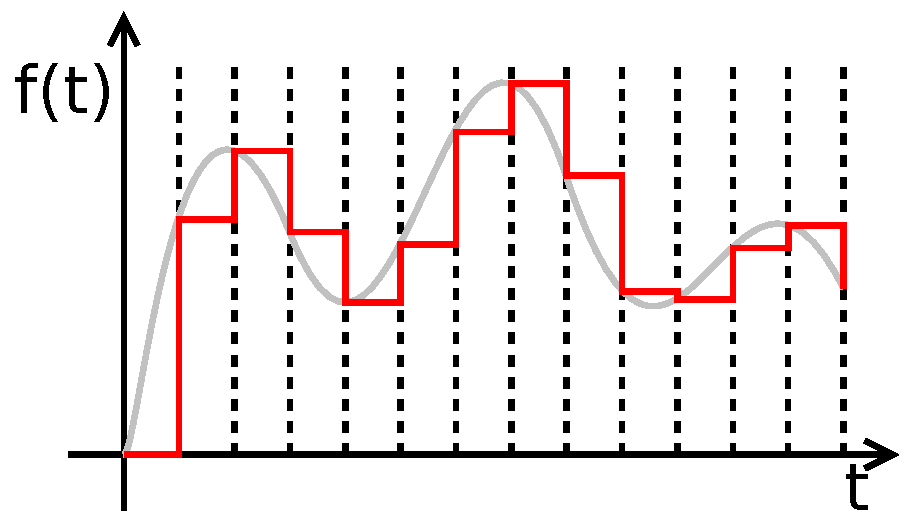
\includegraphics[width=.8\textwidth]{Figures/3_sample_hold_amplifier_quantization.pdf}
	\caption[Sample and Hold function with input function $f(t)$ over time]{Sample and Hold function with input function $f(t)$ over time \cite{sha_pic}}
	\label{fig:3_sha_function}
\end{figure}

\section{Active Filter, DC-Coupling}
\begin{figure}[htbp]
	\centering
	\begin{subfigure}[b]{0.49\textwidth}
		\resizebox{\textwidth}{!}{%
			\begin{circuitikz}
				\tikzstyle{every node}=[font=\normalsize]
				\draw (13,17.25) to[C,l={ \normalsize $C_2$}] (13,15.75);
				\draw (14.5,17.25) to[C,l={ \normalsize $C_3$}] (14.5,15.75);
				\draw (11.75,17.25) to[R,l={ \normalsize $R_2$}] (11.75,15.75);
				\draw [](11.75,17.25) to[short] (14.25,17.25);
				\draw [](14.25,17.25) to[short] (15.25,17.25);
				\draw [](15.25,16.25) to[short] (15.25,15.5);
				\draw [](15.25,15.5) to[short] (17.75,15.5);
				\draw [](17.75,15.5) to[short] (17.75,16.75);
				\draw (16.75,16.75) node[op amp,scale=1, yscale=-1 ] (opamp2) {};
				\draw (opamp2.+) to[short] (15.25,17.25);
				\draw  (opamp2.-) to[short] (15.25,16.25);
				\draw (17.95,16.75) to[short](18.25,16.75);
				\draw (17.75,16.75) to[short, -*] (17.75,16.75);
				\draw [](18.25,16.75) to[short, -o, l=$V_{\mathrm{bias}}$] (18.5,16.75);
				\draw (17.75,15.5) to[C,l={ \normalsize $C_4$}] (17.75,14.5);
				\draw (17.75,14.5) to (17.75,14.25) node[ground]{};
				\draw (10,17.25) to[american voltage source,l={ \normalsize $V_1$}] (10,15.75);
				\draw (10,15.75) to (10,15.5) node[ground]{};
				\draw [](11.75,15.75) to[short] (14.5,15.75);
				\draw (13,15.75) to (13,15.5) node[ground]{};
				\draw (13,15.75) to[short, -*] (13,15.75);
				\draw (10,17.25) to[R,l={ \normalsize $R_1$}] (11.75,17.25);
				\draw (17.75,15.5) to[short, -*] (17.75,15.5);
				\draw (11.75,17.25) to[short, -*] (11.75,17.25);
				\draw (13,17.25) to[short, -*] (13,17.25);
				\draw (14.5,17.25) to[short, -*] (14.5,17.25);
			\end{circuitikz}
		}%
		\caption{Circuit diagram of DC bias circuit}
		\label{fig:3_dc_bias_circuit}
	\end{subfigure}%
	\begin{subfigure}[b]{.49\textwidth}
		\resizebox{\textwidth}{!}{%
			\begin{circuitikz}
				\draw (9.75,15.75) to[sinusoidal voltage source, sources/symbol/rotate=auto,l={ \normalsize $V_{\mathrm{in}}$}] (9.75,17.75);
				\draw (9.75,15.75) to (9.75,15.5) node[ground]{};
				\draw (9.75,17.75) to[C,l={ \normalsize $C_1$}] (11.25,17.75);
				\draw (12.75,17.25) node[op amp,scale=1, yscale=-1 ] (opamp2) {};
				\draw (opamp2.+) to[short] (11.25,17.75);
				\draw  (opamp2.-) to[short] (11.25,16.75);
				\draw (13.95,17.25) to[short](14.25,17.25);
				\draw (11.25,17.75) to[short, -*] (11.25,17.75);
				\draw (14,17.25) to[R,l={ \normalsize $R_3$}] (14,16);
				\draw[] (14,16) to[short] (11.25,16);
				\draw [](11.25,16) to[short] (11.25,16.75);
				\draw [](14.25,17.25) to[short, -o, l=$V_{\mathrm{out}}$] (14.5,17.25);
				\draw [](14,16) to[short] (14,15.5);
				\draw (14,15.5) to[R,l={ \normalsize $R_4$}] (12.75,15.5);
				\draw (12.75,15.5) to[C,l={ \normalsize $C_5$}] (11.75,15.5);
				\draw (11.75,15.5) to (11.5,15.5) node[ground]{};
				\draw (14,17.25) to[short, -*] (14,17.25);
				\draw [](11.25,17.75) to (11.25,18) node[vcc]{\normalsize $V_{\mathrm{bias}}$};
			\end{circuitikz}
		}%
		\caption{Circuit diagram of \gls{hp}, \gls{prf} and Wall filter}
		\label{fig:3_prf_wall_diagram}
	\end{subfigure}
\end{figure}
Finally, the signal should be DC coupled for sampling and filtered using an active \gls{hp} filter to remove unwanted PRF frequency and wall frequency. For generating a DC bias voltage, the circuit in \cref{fig:3_dc_bias_circuit} is used. Here, a voltage divider is coupled with some stabilising capacitors and a voltage follower to output a stable output. In the circuit diagram in \cref{fig:3_prf_wall_diagram}, a \gls{hp} filter is used as a combined \gls{prf} and Wall-filter in conjunction with a \qty{2}{\decibel} gain amplification to maximize the dynamic range of the \gls{adc} measurements from \qtyrange{0}{3.3}{\volt}. In the diagram, $V_{bias}=\qty{1.65}{\volt}$, which is half of the \gls{adc} dynamic range of \qtyrange{0}{3.3}{\volt}, and $v_{\mathrm{in}}$ is the input signal to the filter from the output of the sample-and-hold amplifier. To get a \qty{1.65}{\volt} DC-bias, a voltage-follower op-amp configuration is used with a voltage divider input on the supply voltage of \qty{5}{\volt}, outlined in \cref{eq:3_dc_couple_voltage}.
\begin{equation} \label{eq:3_dc_couple_voltage}
	V_{\mathrm{dc}}= V_{\mathrm{cc}} \cdot \frac{R_{2}}{R_{1}+R_{2}} = \qty{5}{\volt} \cdot \frac{\qty{5}{\kilo\ohm}}{\qty{10}{\kilo\ohm}+\qty{5}{\kilo\ohm}} = \qty{1.66}{\volt}
\end{equation}
For the \qty{2}{\decibel} gain, a non-inverting amplifier configuration is used, expressed by \cref{eq:3_dc_couple_gain}.
\begin{equation} \label{eq:3_dc_couple_gain}
	G_{\unit{\decibel}} = \frac{V_{\mathrm{out}}}{V_{\mathrm{in}}} = 20\cdot \log_{10} \left(1 + \frac{R_3}{R_4} \right) = 20\cdot \log_{10} \left( 1 + \frac{\qty{40}{\kilo\ohm}}{\qty{150}{\kilo\ohm}} \right) = \qty{2.05}{\decibel}
\end{equation}
A SPICE simulation was implemented and can be seen in \cref{fig:app_ltspice_dc_coupler}. From this simulation model, a small signal analysis as well as a transient analysis was conducted. The resulting small signal analysis can be seen in \cref{fig:3_dccoupler_sim_ac} and the transient analysis can be seen in \cref{fig:3_dccoupler_sim_transient} and confirms the expected result.
\begin{figure}[htbp]
	\centering
	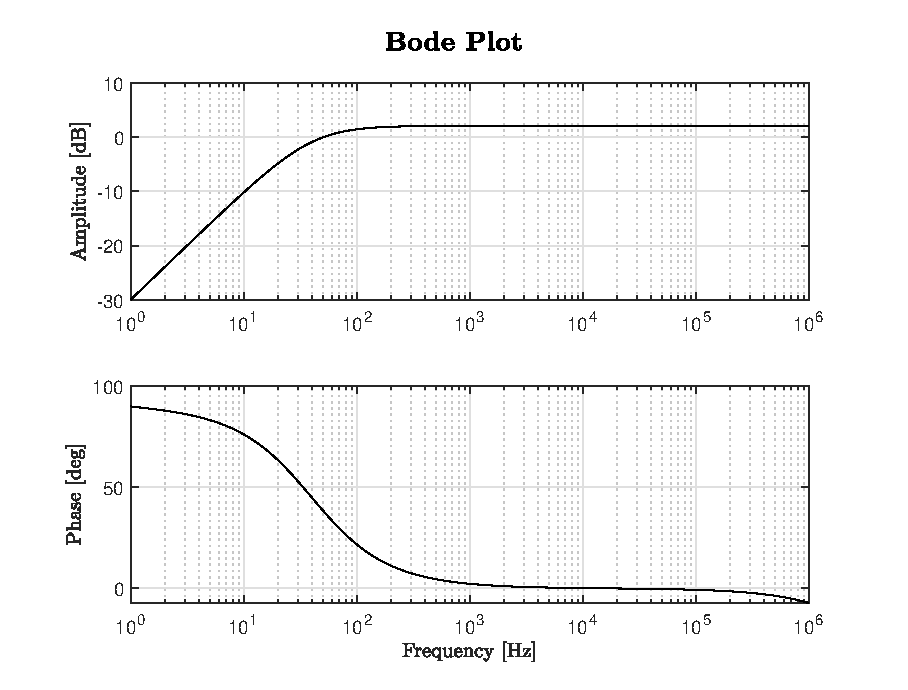
\includegraphics[width=.8\textwidth]{Figures/3_dc_coupler_sim.eps}
	\caption{Small-signal analysis of DC-Coupling filter circuit}
	\label{fig:3_dccoupler_sim_ac}
\end{figure}
\begin{figure}[htbp]
	\centering
	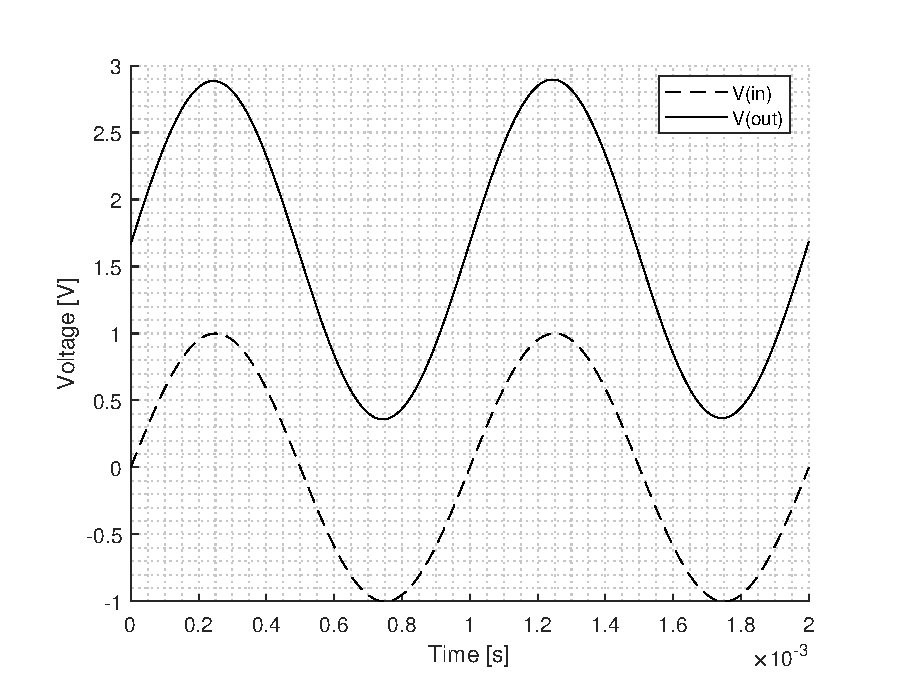
\includegraphics[width=.8\textwidth]{Figures/3_dc_coupler_sim_transient.eps}
	\caption{Transient analysis of DC-Coupling filter circuit}
	\label{fig:3_dccoupler_sim_transient}
\end{figure}

\section{Digital Signal Processor}
In the \gls{dsp} system, the function is to turn a waveform into a humanly readable velocity metric by performing an \gls{fft} of the input signal captured from the output of the active filter of the previous section. Since DSP devices are programmable \gls{dc} devices of typically \qtyrange{3.3}{5}{\volt}, it is vital that the input signal is \gls{dc}-coupled. Since the input signal is relatively low frequency, most \gls{adc} interfaces should be sufficient to capture a frequency window of less than \qty{10}{\kilo\hertz}.